\documentclass[a4paper, 9pt]{article}
\title{FISICA TECNICA - riassunto}
  
\author{Federico Mainetti Gambera}
\usepackage{amsmath}
\usepackage{amssymb}
\usepackage{graphicx}
\usepackage[italian]{babel}
\usepackage{import}
\usepackage{xifthen}
\usepackage{pdfpages}
\usepackage{transparent}
\usepackage{xcolor}
\usepackage{cancel}
\usepackage[a4paper,left=35mm,top=26mm,right=26mm,bottom=15mm]{geometry}
\usepackage{color}
\usepackage{tcolorbox}
\usepackage{hyperref}
\usepackage{makeidx}
\makeindex
\definecolor{lightgray}{gray}{0.75}
\renewcommand{\familydefault}{\sfdefault}
\newenvironment{rcases}
  {\left.\begin{aligned}}
  {\end{aligned}\right\rbrace}
\newcommand{\incfig}[1]{%
    \def\svgwidth{\columnwidth}
    \import{../images/}{#1.pdf_tex}
}
\usepackage{sectsty}
\usepackage{xcolor}
\definecolor{myblue}{RGB}{66, 151, 255}
\sectionfont{\color{myblue}\Huge}
\subsectionfont{\color{myblue}\huge}
\subsubsectionfont{\color{myblue}\large}
\begin{document}
    \maketitle
    \tableofcontents{}
    \newpage
    \part{Teoria}
    \newpage
    \url{../pdf/Lezioni/L01-Introduzione (1).pdf}
    \section{L01-Introduzione}
\subsection{Introduzione}
La \textbf{termodinamica} è la scienza che studia \textbf{l’energia}, la \textbf{materia} e le \textbf{leggi} che governano le loro interazioni (scambi).
\subsubsection{Sistema termodinamico}
Il sistema termodinamico è inteso come porzione di spazio limitata da un \textbf{contorno} che lo racchiude completamente (il contorno è costituito da una superficie reale o immaginaria, rigida o deformabile).\newline
\newline
Tutto ciò che è esterno al sistema termodinamico è il \textbf{mondo esterno} e quando il mondo esterno è di massa infinita viene chiamato \textbf{ambiente}.\newline
\newline
I termini \textbf{serbatoio}, \textbf{sorgente} o \textbf{pozzo} fanno riferimento ad ambienti che interagiscono con il sistema termodinamico.\newline
\newline
Un \textbf{sistema composto} è un insieme di sistemi e sottosistemi a massa finita e/o infinita.\newline
\newline
Il sistema può essere \textbf{monocomponente} (sostanza pura o miscela di sostanze pure in rapporto fisso, quale ad esempio l'aria) o \textbf{policomponente} cioè composto da più componenti.\newline
\newline
Ogni sistema monocomponente può essere in diversi \textbf{stati di aggregazione} (solido, liquido, aeriforme). I sistemi saranno \textbf{monofase} o \textbf{polifase}.
\subsubsection{Il sistema semplice}
\begin{itemize}
    \item Chimicamente e fisicamente omogeneo ed isotropo;
    \item non soggetto a campi gravitazionali, elettrici o magnetici;
    \item chimicamente inerte
    \item esente da effetti di superficie per via delle grandi dimensioni.
\end{itemize}
\subsection{Stato di equilibrio}
Lo \textbf{stato di equilibrio} è il particolare stato cui perviene spontaneamente il sistema isolato.\newline
\newline
E' \textbf{ripoducibile} e \textbf{descrivibile} da poche proprietà del sistema stesso.
\subsubsection{Variabili termodinamiche}
Il sistema all’equilibrio è compiutamente descritto attraverso un numero ristretto di \textbf{variabili termodinamiche} (anche dette grandezze o proprietà di stato, variabili o funzioni di stato).\newline
\newline
Le grandezze si dividono in:
\begin{itemize}
    \item \textbf{Grandezza intensiva}: valore \textbf{non dipende} dall'estensione del sistema (per esempio temperatura, pressione, densità). Ne
    consegue che lo stato interno del corpo non dipende dalla sua estensione.
    \item \textbf{Grandezza estensiva}: valore \textbf{dipende} dall'estensione del sistema (per esempio massa, volume). La grandezza
    estensiva è additiva e di conseguenza il suo valore riferito ad un sistema
    risulta somma dei valori relativi ai sottosistemi che lo compongono.
    \item \textbf{Grandezza estensiva specifica}: grandezza estensiva divisa per un'altra grandezza estensiva (tipicamente massa o numero di moli, per esempio $v = \frac{V}{M}$).
\end{itemize}
\begin{center}
    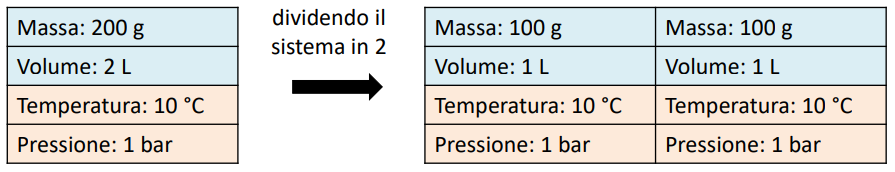
\includegraphics[height=2cm]{../L01/img1.PNG}
\end{center}
Le grandezze estensive specifiche ed intensive vengono normalmente usate per descrivere lo stato di equilibrio di un sistema termodinamico.\newline
\newline
Indicheremo le grandezze estensive, riferite cioè all'intera massa, con le lettere maiuscole e le estensive specifiche con le lettere minuscole.\newline
\newline
\textbf{Leggedi Duhem}:\newline
«Nel caso di sistema monocomponente, il numero di parametri termodinamici intensivi o estensivi specifici indipendenti atti a descrivere compiutamente lo stato interno di equilibrio è due.»
\subsubsection{Regola di Gibbs}
La differenza di ruolo tra grandezza estensiva specifica ed intensiva è messa in evidenza dalla regola di Gibbs
\[
    V = C+2-F
\]
$C$: numero di componenti;\newline
$F$: numero di fasi;\newline
$V$: numero di variabili intensive indipendenti utilizzabili.\newline
\newline
Concludendo la coppia intensiva-intensiva è sufficiente a descrivere il sistema monocomponente monofase, mentre per il sistema monocomponente bifase sarà necessaria la coppia intensiva-estensiva e per il sistema monocomponente trifase sarà necessaria una coppia estensiva-estensiva. 
\subsection{Tipologie di sistemi termodinamici}
Tipologie di \textbf{contorni}:
\begin{center}
    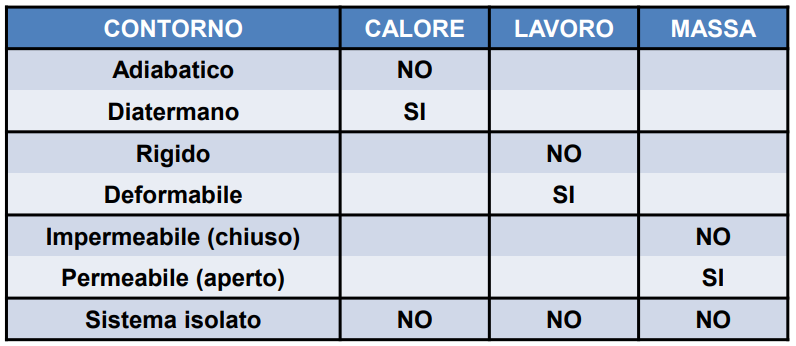
\includegraphics[height=4cm]{../L01/img2.PNG}
\end{center}
Sistema \textbf{aperto} e \textbf{chiuso}:\newline
Si parlerà di sistema chiuso se il contorno del sistema non consente scambi di massa con l’esterno; in tal caso la massa del sistema rimane costante mentre sono possibili scambi di energia sotto forma di lavoro e/o di calore con l’ambiente circostante. Un caso particolare di sistema chiuso è costituito dal sistema isolato il quale non ha scambi di energia con l’esterno.\newline
Il sistema viene inoltre definito aperto se può scambiare con l'ambiente massa.
\begin{center}
    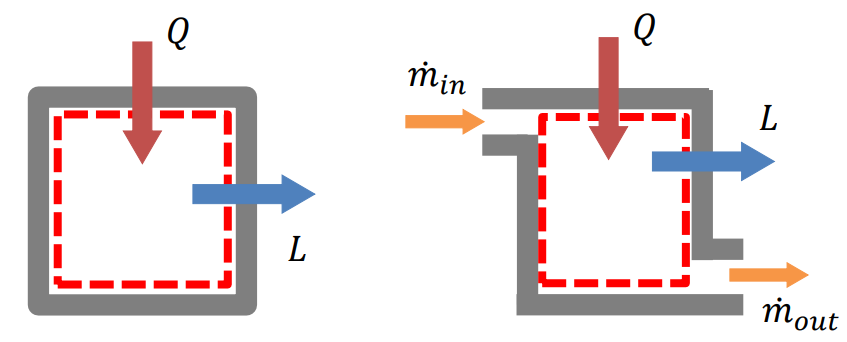
\includegraphics[height=3cm]{../L01/img3.PNG}
\end{center}
\subsection{Trasformazioni termodinamiche}
L’\textbf{insieme degli stati intermedi} successivi, tra lo stato iniziale e finale, a seguito di una variazione del sistema termodinamico, definisce la \textbf{trasformazione termodinamica}.\newline
\newline
Le trasformazioni termodinamiche si dividono in:
\begin{itemize}
    \item \textbf{Quasi-statica} o \textbf{internamente reversibile}: Costituita da una successione di stati di equilibrio; può non essere reversibile. 
    \item \textbf{Reversibile}: Se percorsa in senso inverso, riporta il sistema e ambiente nello stasto iniziale. Per trasformazione reversibile si intende spesso una trasformazione lenta.
    \begin{itemize}
        \item Traformazione \textbf{internamente reversibile}: nessuna irreversibilità si verifica all'interno del sistema.
        \item Trasformazione \textbf{esternamente reversibile}: nessuna irreversibilità si verifica all'esterno del sistema.
        \item Trasformazione \textbf{totalmente reversibile (o reversibile)}: non implica alcuna irreversibilità sia all'interno sia all'esterno del sistema.
    \end{itemize}
    \item \textbf{Irreversibile}: Trasformazione in parte o per intero non reversibile. Non è rappresentabile su un diagramma di stato. Per trasformazione irreversibile si intende spesso una trasformazione veloce.
    \item \textbf{Chiusa} o \textbf{ciclica}: Gli estremi della trasformazione coicidono.
    \item \textbf{Elementare}: Se una delle grandezze di stato si manitiene costatne durante la traformazione.
\end{itemize}
\subsection{Equazione di stato nelle coordinate P,v,T}
\textbf{equazione di sato}:
\[
    f(P,v,T) = 0
\]
In molti casi, l'equazione di stato è ignota.\newline
\newline
L’ \textbf{equazione di stato} di un \textbf{sistema semplice} è rappresentata in uno spazio cartesiano tridimensionale da una superficie detta «\textbf{superficie di stato}», luogo dei punti rappresentativi di \textbf{tutti i possibili stati} termodinamici di \textbf{equilibrio}.
\begin{center}
    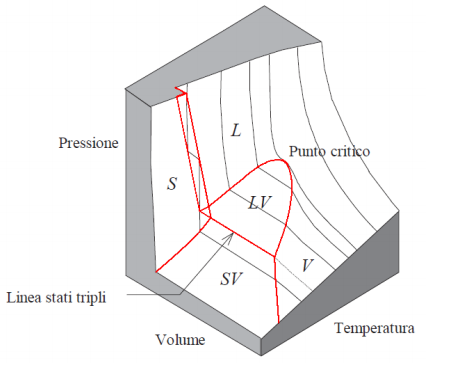
\includegraphics[height=5cm]{../L01/img4.PNG}
\end{center}
Lo stato termodinamico (punto appartenente alla superficie di stato) può anche essere geometricamente
rappresentato da un punto su un piano cartesiano sui cui assi vi sono due delle tre variabili prescelte.\newline
In particolare si possono realizzare piani termodinamici in coordinate (P,v), (P,T) e (T,v).
\subsubsection{Equazione di stato per i gas ideali}
\[
    PV=NRT
\]
$P$: pressione [$Pa$]\newline
$V$: volume [$m^3$]\newline
$N$: moli [$kmole$]\newline
$T$: temperatura [$K$]\newline
$R$: costante universale dei gas ideali $\rightarrow R = 8314 [J/(kmole \; K)]$\newline
Oppure:
\[
    PV = MR^*T
\]
$M$: massa [$kg$]\newline
$M_m$: massa molare [$kg/kmole$]\newline
$R^*$: costante caratteristica del gas considerato $\rightarrow R^* = \frac{R}{M_m}$
\begin{center}
    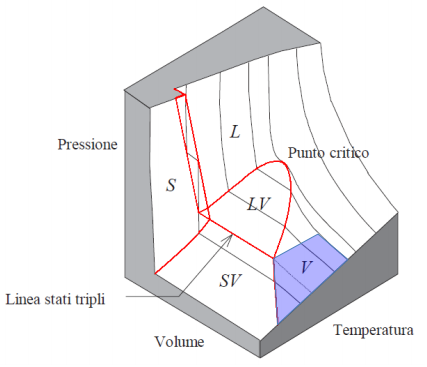
\includegraphics[height=5cm]{../L01/img5.PNG}
\end{center}
\subsubsection{Equazione di stato per i gas reali}
Modello di equazione di stato più complesso per descrivere il comportamento di gas in condizioni di \textbf{temperatura} e \textbf{pressioni elevate}.\newline
\newline
Equazione di van der Waals:
\[
    \left(P + \frac{a}{v_m^2}\right)(v_m - b) = RT
\]
Ove $a$ e $b$ sono caratteristiche del particolare gaas considerato:
\begin{center}
    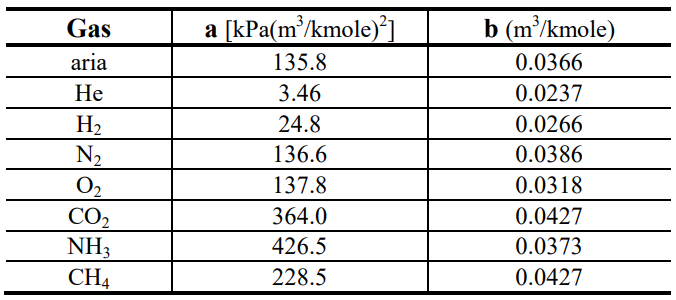
\includegraphics[height=3cm]{../L01/img8.PNG}
\end{center}
\begin{center}
    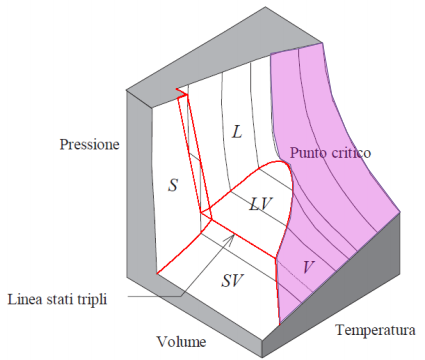
\includegraphics[height=5cm]{../L01/img6.PNG}
\end{center}
\subsubsection{Equazione di stato per liquidi e solidi}
\[
    dv = \beta v dT - K_T v dP
\]
\[
    \begin{matrix}
        \text{Coefficiente di dilatazioen termica isobaro}\; & \beta = \frac{1}{v}\left(\frac{\delta v}{\delta T}\right)_P\\
        \text{Coefficiente di comprimibilità isotermo}\; & K_T = - \frac{1}{v}\left( \frac{\delta v}{ \delta P} \right)_T
    \end{matrix}
\]
Siccome $\beta$ e $K_T$ possono essere considerati costanti per ampi intervalli di temperatura e di pressione, la precedente relazione differenziale è integrabile e lo stato calcolabile.
\begin{center}
    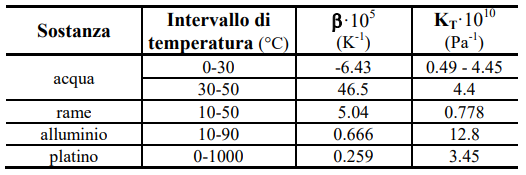
\includegraphics[height=3cm]{../L01/img9.PNG}
\end{center}
\begin{center}
    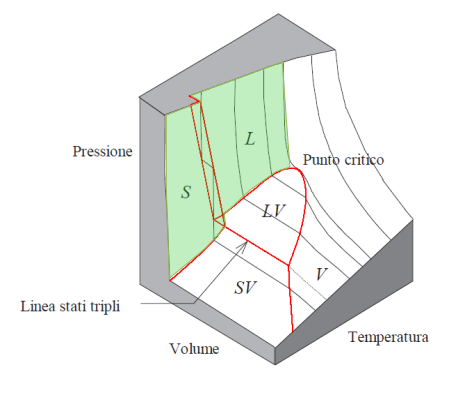
\includegraphics[height=5cm]{../L01/img7.PNG}
\end{center}
Un modello semplificato è quello per \textbf{liquidi e solidi incomprimibili}, in cui si considera $v =$ costante.
\subsection{NOTE SUGLI ESERCIZI}
    \newpage
    \url{../pdf/Lezioni/L02-Principi di conservazione.pdf}
    \section{L01-Principi di conservazione}
    \newpage
    \url{../pdf/Lezioni/L03-Trasformazioni-con-annotazioni.pdf}
    \section{L03-Trasformazioni}
Per variabile di stato si intende una grandezza che dipende dallo stato del sistema, viceversa variabili come il lavoro e il calore (che non sono di stato) non dipendono dallo stato del sistema, ma bensì dal percorso che hanno seguito per raggiungere quel determinato stato.
\subsection{Il lavoro termodinamico}
In un dispositivo cilindro-pistone, uno squilibrio di forze infinitesimo tra forze esterne e forza interna ($P \cdot A$) provoca uno spostamento infinitesimo del pistone a cui corrisponde un \textbf{lavoro}
\[
    \delta L^\rightarrow  = P A ds = P \cdot dV
\]
\begin{center}
    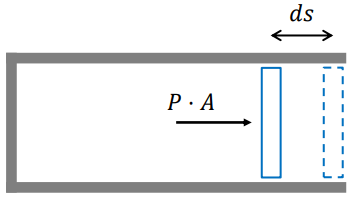
\includegraphics[height=3cm]{../L03/img1.PNG}
\end{center}
In termini di grandezze specifiche, la relazione diventa
\[
    \delta l^\rightarrow = P \cdot dv
\]
Quando il sistema evolve da uno stato \textbf{iniziale} (i) ad uno stato \textbf{finale} (f) attraverso una successione di \textbf{stati di equilibrio}, allora sarà possibile esprimere una legge, detta \textbf{equazione della trasformazione}, tra le variabili di stato $P$ e $v$ e la integrazione di $P dv$ rappresenterà il lavoro scambiato durante la trasformazione.\newline
Il lavoro termodinamico è dunque calcolabile come
\[
    l^\rightarrow = \int_{i}^{f}Pdv
\]
che è un integrale calcolabile solo se si conosce la funzione $P = P (v)$ detta equazione della trasformazione, che si può ricavare dall'equazione di stato.
\subsubsection{Il lavoro termodinamico nelle trasformazioni reversibili e irreversibile}
Nel caso di trasformazione \textbf{reversibile} in un cilindro-pistone la pressione interna è sempre omogenea all'interno del cilindro.
\begin{center}
    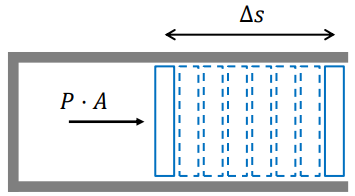
\includegraphics[height=2cm]{../L03/img2.PNG}
\end{center}
Nel caso di trasformazione \textbf{irreversibile} in un cilindro-pistone la pressione interna non è omogenea all'interno del cilindro. Quindi per ricavare la forza applicata al pistone si usa la pressione dell'ambiente esterno che agisce sul pistone.
\begin{center}
    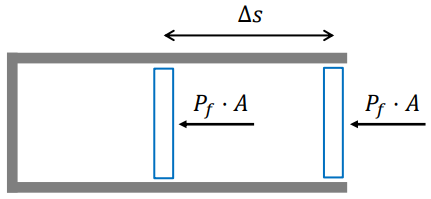
\includegraphics[height=2cm]{../L03/img3.PNG}
\end{center}
\ \newline
\newline
Solitamente il lavoro reversibile è maggiore del lavoro irreversibile, come si vede bene dal seguente grafico:
\begin{center}
    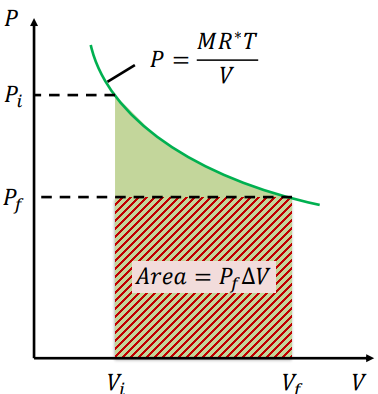
\includegraphics[height=5cm]{../L03/img4.PNG}
\end{center}
L'area verde insime all'area a linee rosse (cioè tutta quella sottesa alla curva) rappresenta il lavoro nel caso di trasformazione reversibile, la sola area a linee rosse rappresenta, invece, il lavoro nel caso di trasformazione irreversibile.
\subsubsection{Il lavoro termodinamico di un ciclo}
Un ciclo è un trasformazione che termina con lo stato iniziale. In funzione di come avviene il ciclo, orario o antiorario per esempio, avremo che il lavoro uscente dal sistema è positivo o negativo. Nel
piano $PV$ chiamiamo macchine a \textbf{ciclo diretto} (motrici) quelle che eseguono trasformazioni in senso orario, mentre chiameremo macchine a \textbf{ciclo inverso} (operatrici) quelle che eseguono trasformazioni in senso antiorario.
\begin{center}
    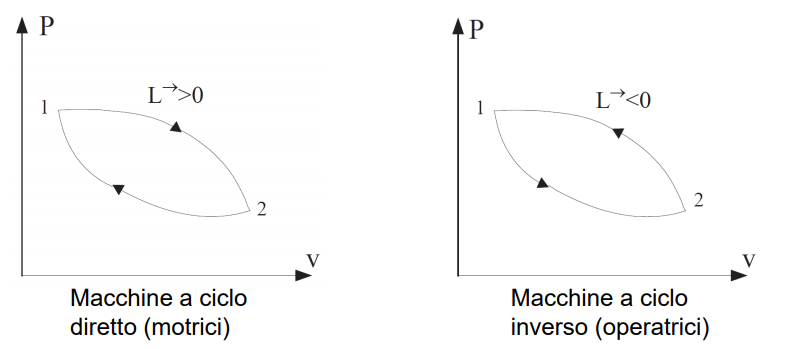
\includegraphics[height=3cm]{../L03/img5.PNG}
\end{center}
\subsection{Il calore}
\textbf{Capacità termica}: è il rapporto fra il calore fornito al sistema e la variazione di temperature del sistema stesso
\[
    C_x = \left(\frac{\delta Q^\leftarrow }{d T}\right)_x
\]
\textbf{Calore specifico}: è il rapporto tra la capacità termica del sistema e la sua massa
\[
    c_x = \frac{1}{M}\left(\frac{\delta Q^\leftarrow }{dT}\right)_x
\]
I calori specifici possono essere interpretati come \textbf{derivate parziali di funzioni termodinamiche}.\newline
\newline
Il pedice $x$ precisa la \textbf{trasformazione} lungo la quale viene scambiato il calore $\delta Q$. Vediamo i casi in cui $x$ è la pressione e $x$ è il volume.
\subsubsection{Calori specifici a volume costante $c_V$}
\[
    c_V =\frac{1}{M}\left(\frac{\delta Q^\leftarrow }{dT}\right)_V = \left(\frac{\delta q^\leftarrow }{dT}\right)_V
\]
Partendo dal primo principio della termodinamica e dalla definizione di lavoro data precedentemente si può scrivere che $\delta q^\leftarrow  = d u + Pdv$ e che quindi $\delta q^\leftarrow  = \left(\frac{\delta u}{\delta T}\right)_vdT + \left(\frac{\delta u}{\delta T}\right)_T dv + Pdv$, e proseguendo considerando il fatto che il volume è costante ricaviamo che $\delta q^\leftarrow  = \left(\frac{\delta u}{\delta T}\right)_VdT$, da cui ricaviamo che 
\[
    c_V = \left( \frac{\delta u}{\delta T} \right)_V
\]
Siccome è una \textbf{derivata di una funzione di stato}, può in generale essere espresso come funzione di una coppia di variabili termodinamiche (in particolare della coppia $T$,$P$):
\[
    c_V = c_V(T,P)
\]
\subsubsection{Calori specifici a pressione costante $c_P$}
\[
    c_P =\frac{1}{M}\left(\frac{\delta Q^\leftarrow }{dT}\right)_P = \left(\frac{\delta q^\leftarrow }{dT}\right)_P
\]
Per lavorare sul calore specifico a pressione costante dobbiamo introdurre la funzione di stato \textbf{entalpia}, che esprime la quantità di energia che un sistema può scambiare con l'ambiente ed è definita come
\[
    h = u + Pv
\]
Per le trasformazioni che avvengono a pressione costante, la variazione di entalpia è uguale al calore scambiato dal sistema con l'ambiente esterno. Col suo differenziale possiamo riscrivere il primo principio come $dh = du + vdP + Pdv$, da cui, ricordando che siamo a pressione costante, ricaviamo che $\delta q^\leftarrow = dh - vdP = \left(\frac{\delta h}{\delta T}\right)_P dT + \left(\frac{\delta h}{\delta T}\right)_T dP - vdP$, e quindi $\delta q^\leftarrow  =  \left(\frac{\delta h}{\delta T}\right)_P dT$, da cui ricaviamo che
\[
    c_P =  \left(\frac{\delta h}{\delta T}\right)_P
\]
Siccome è una \textbf{derivata di una funzione di stato}, può in generale essere espresso come funzione di una coppia di variabili termodinamiche (in particolare della coppia $T$,$P$): 
\[
    c_P = c_P(T,P)
\]
\subsubsection{$c_V$ e $c_P$ per i gas ideali}
Per un gas ideale la variazione di energia interna e l'entalpia sono funzioni della sola temperatura $u = u(T)$ e $h = h(T)$, per cui i calori specifici da derivate parziali diventano derivate esatte:
\[
    c_V = c_V(T) = \left(\frac{\delta u}{\delta T}\right)
\]
\[
    c_P = c_P(T) = \left( \frac{\delta h}{ \delta T}\right)
\]
Vale inoltre la \textbf{realzione di Mayer}
\[
    c_P = c_V + R^*
\]
\subsubsection{$c_V$ e $c_P$ per i gas perfetti}
Per i gas ideali i calori specifici dipendono dalla temperatura, ma questa relazione di dipendenza è molto debole, per cui in intervalli ristretti di temperatura i calori specifici si ritengono spesso costanti: in questo caso il gas viene definito \textbf{perfetto}.\newline
\newline
Per calcolare i calori specifici si usano le seguenti relazioni:
\begin{itemize}
    \item \textbf{Gas monoatomico} ($He$, $Ar$)
    \[
        c_v = \frac{3}{2}R^*; \;\;\;\;\;\;\;\;\;\;\;\;\;\;\;c_P = \frac{5}{2}R^*
    \]
    \item \textbf{Gas biatomico o poliatomico lineare}: ($N_2$, $O_2$, $CO_2$)
    \[
        c_v = \frac{5}{2}R^*; \;\;\;\;\;\;\;\;\;\;\;\;\;\;\;c_P = \frac{7}{2}R^*
    \]
    \item \textbf{Gas poliatomico non lineare}: ($CH_4$)
    \[
        c_v = \frac{6}{2}R^*; \;\;\;\;\;\;\;\;\;\;\;\;\;\;\;c_P = \frac{8}{2}R^*
    \]
\end{itemize}
\subsubsection{$c_V$ e $c_P$ per i liqudi (e solidi) incomprimibili ideali}
\[
    c_V = c_P = c(T)
\]
\subsubsection{$c_V$ e $c_P$ per i liqudi (e solidi) incomprimibili perfetti}
\[
    c_V = c_P = c = \text{costante}
\]
\subsection{Le trasformazioni politropiche}
\subsubsection{Trasformazione politropica per un gas ideale}
\subsubsection{Trasformazione politropica per un gas perfetto}
\subsubsection{Espressioni della politropica}
\subsubsection{Politropiche per trasformazioni elementari}
\subsubsection{Lavoro lunga una generica politropica}
\subsubsection{Politropiche nel diagramma T-S}
\subsection{Calcolo delle grandezze termodinamiche}
\dots
    \newpage
    \url{../pdf/Lezioni/L04-Sistemi bifase-con-annotazioni.pdf}
    \section{L04-Sistemi bifase}
\subsection{Sistema eterogeneo}
Un sistema \textbf{omogeneo} è un sistema con un solo stato di aggregazione.\newline
\newline
Un sistema \textbf{eterogeneo} è un sistema con più stati di aggregazione.\newline
\newline
Un sistema \textbf{monocomponente} è un sistema con una sola sostanza al suo interno.\newline
\newline
Un sisteam \textbf{multicomponente} è un sistea con più sostanze al suo interno.\newline
\newline
Le generica \textbf{grandezze estensive specifiche} $e$ di un sistema eterogeneo costituito da due stati di aggregazione $\alpha$ e $\beta$ possono essere rappresentate come \textbf{media pesata sulle masse} dei valori delle grandezze estensive specifiche delle singole fasi:
\[
    e = \frac{M_\alpha}{M}e_{\alpha} + \frac{M_\beta}{M}e_\beta
\]
\ \newline
Si definisce \textbf{frazione massica} le proporzioni di massa in uno stato di aggregazione rispetto alla massa complessiva. Per esempio in un generico sistema eterogeneo con due stati di aggregazione $\alpha$ e $\beta$:
\[
    x_\alpha = \frac{M_\alpha}{M} \;\;\;\;\;\;\;\;\;\;\;\;\;\;\; x_\beta = \frac{M_\beta}{M}
\]
Ricordiamo inoltre che 
\[
    x_\alpha + x_\beta = 1
\]
e che una generica grandezza estensiva specifica può quindi essere espressa come
\[
    e = x_\alpha e_\alpha + x_\beta e_\beta = (1-x_\beta)e_\alpha + x_\beta e_\beta
\]
\subsubsection{Regola di gibs per sistemi eterogenei}
\textbf{Regola di Gibbs}:
\[
    V = C + 2 -F
\]
$V$: numero di \textbf{variabili intensive indipendenti} utilizzabili per descrivere il generico stato di equilibrio.\newline
$C$: numero di componenti.\newline
$F$: numero di fasi.
\begin{itemize}
    \item Per il generico sistema \textbf{monocomponente e monofase} $V =2$, quindi per descrivere uno stato di equilibrio è sufficiente una coppia intensiva-intensiva (per esempio $P$ e $T$).
    \item Per il generico sistema \textbf{monocomponente bifase} $V =1$, quindi per descrivere lo stato termodinamico è necessaria una coppia intensiva-estensiva oppure un coppia estensiva-estensiva:\newline
    $(P,v) \;\; (T,v) \;\; (P,u) \;\; (T,u) \;\; (P,h) \;\; (T,h) \;\; (P,s) \;\; (T,s) \;\; (v,u) \;\; (v,h) \;\; (v,s) \;\; (u,h) \;\; (u,s) \;\; (h,s)$
    \item Per il generico sistema \textbf{monocomponente trifase} $V=0$, quindi per descirvere uno stato di equilibrio è necessaria un coppia estensiva-estensiva:\newline
    $(v,u) \;\; (v,h) \;\; (v,s) \;\; (u,h) \;\; (u,s) \;\; (h,s)$
\end{itemize}
\subsubsection{Transizione di fase}
Una \textbf{transizione di fase}:
\begin{itemize}
    \item è il passaggio da uno stato di aggregazione ad un altro;
    \item avviene a pressione (e temperatura) costatne.
\end{itemize}
\ \newline
Definiamo l'\textbf{entalpia di transizione} come la quantità di energia necessaria per passare da uno stato a un altro:
\[
    dh = \delta q^\leftarrow 
\]
\subsubsection{Sistemi eterogenei monocomponente}
Possibili configurazioni:
\begin{itemize}
    \item \textbf{Stati monofase}:
    \begin{itemize}
        \item Solido
        \item Liquido 
        \item Aeriforme (Gas)
    \end{itemize}
    \item \textbf{Stati bifase}:
    \begin{itemize}
        \item Coesistenza di solido e liquido
        \item Coesistenza di solido e aeriforme (vapore)
        \item Coesistenza di liquido e aeriforme (vapore)
    \end{itemize}
    \item \textbf{Stati tripli}:
    \begin{itemize}
        \item Coesistenza di solido, liquido e aeriforme (vapore)
    \end{itemize}
\end{itemize}
Terminologia:
\begin{itemize}
    \item \textbf{Liquido sottoraffreddato}: liquido non in porcinto di evaporare (temperatura di sistema sotto temperatura di saturazione)
    \item \textbf{Liquido saturo}: liquido in procinto di evaporare (liquido a temperatura di saturazione)
    \item \textbf{Vapore saturo}: vapore in condizioni di incipiente condensazione (gas a temperatura di saturazione)
    \item \textbf{Vapore surriscaldato}: vapore non in procinto di condensare (temperatura di sistema sopra temperatura di saturazione)
    \item \textbf{Temperatura di saturazione}: temperatura alla quale una sostanza pura comincia ad evaporare (se è un liquido) oppure condensare (se è un gas), fissata la pressione.
\end{itemize}
\subsection{Diagramma di stato P-v-T}
\subsubsection{terminologia}
\begin{center}
    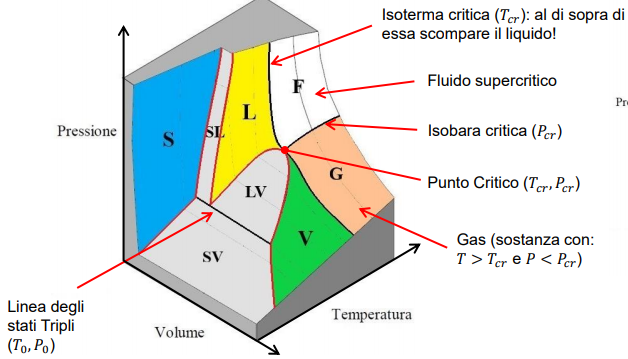
\includegraphics[height=5cm]{../L04/img2.PNG}
\end{center}
\begin{center}
    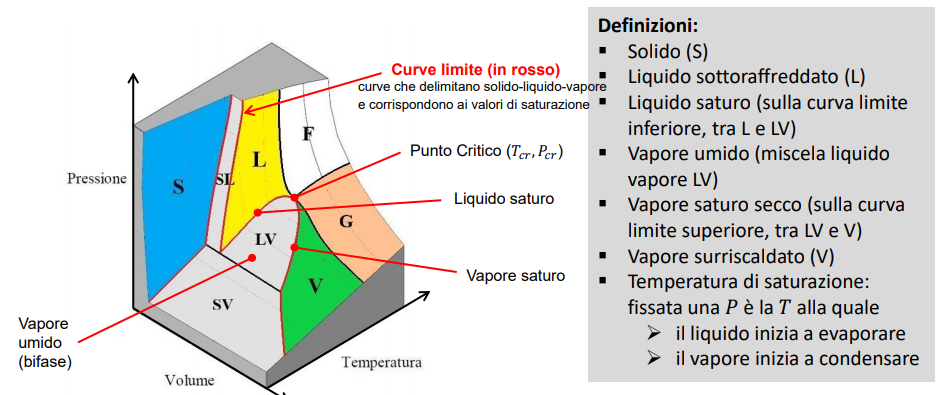
\includegraphics[height=5cm]{../L04/img1.PNG}
\end{center}
\subsubsection{Proiezione del diagramma P-v-T in un grafico P-T}
\begin{center}
    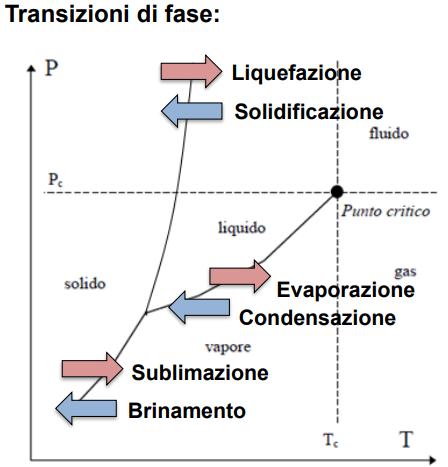
\includegraphics[height=7cm]{../L04/img3.PNG}
\end{center}
\subsubsection{Gas}
Fluido a $P< P_{cr}$ e $T> T_{cr}$ che non può essere liquefatto attraverso una trasformazione di compressione isoterma:
\begin{center}
    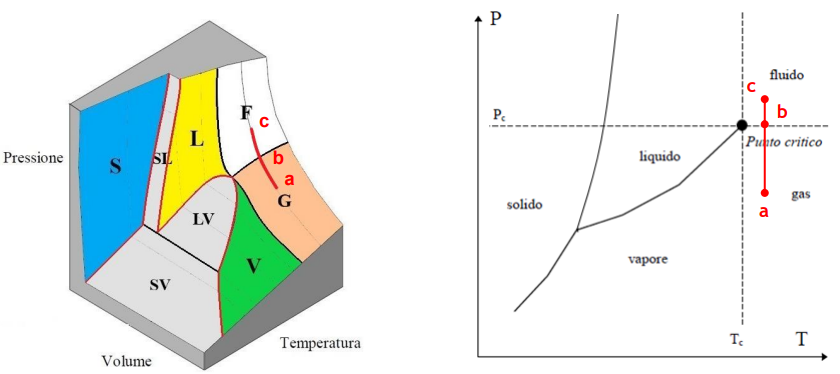
\includegraphics[height=7cm]{../L04/img4.PNG}
\end{center}
\subsubsection{Trasformazione isobara}
\begin{center}
    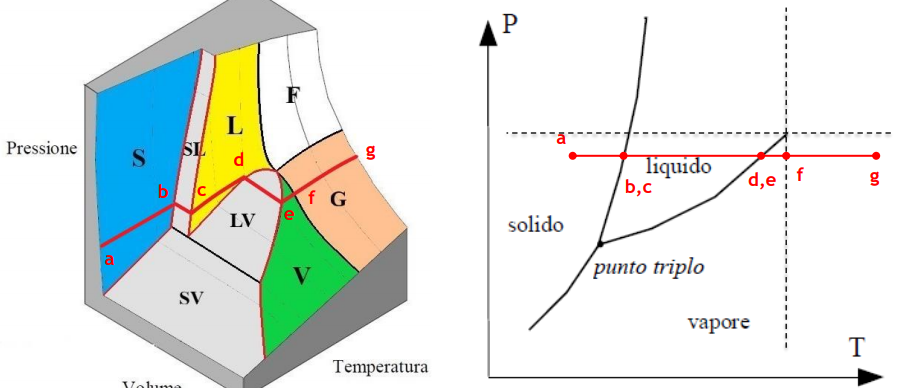
\includegraphics[height=6cm]{../L04/img6.PNG}
\end{center}
\begin{center}
    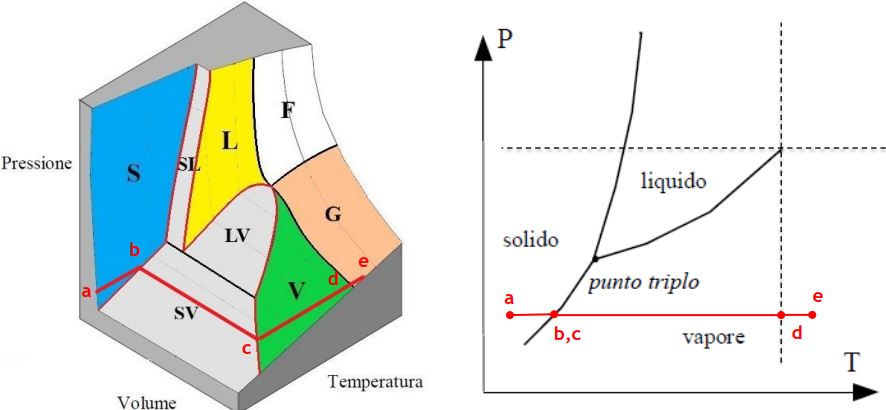
\includegraphics[height=7cm]{../L04/img5.PNG}
\end{center}
\subsubsection{Traformazione isoterma}
\begin{center}
    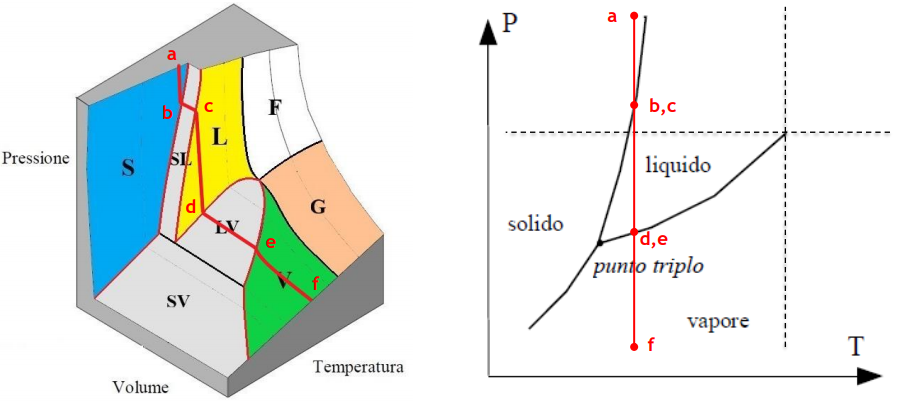
\includegraphics[height=6cm]{../L04/img7.PNG}
\end{center}
\subsubsection{Proiezione del diagramma P-v-T in un grafico P-s e P-h}
Uno dei problemi del proiettare la superficie di stato ne ldiagramm $P-T$, è che difficilmente riusciamo a rappresentare le transizioni di fase, perchè, per esempio le zone SL e LV corrispondono soltanto a un punto. Perciò il diagramma $P-T$ è poco utili per rappresentare i cambi di stato. Per ovviare a ciò dobbiamo fare diverse proiezioni della superficie di stato, rispetto a una coppia di grandezze $(P,v)$, per esempio:
\begin{center}
    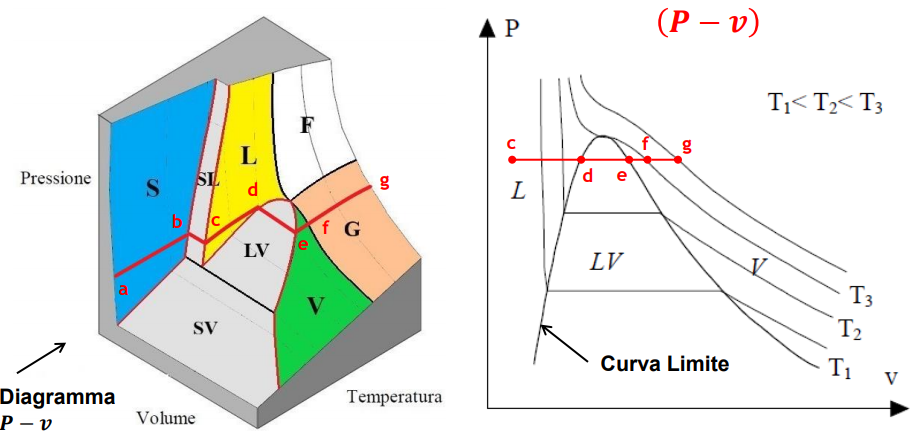
\includegraphics[height=6cm]{../L04/img8.PNG}
\end{center}
Una soluzione a questo problema di rappresentazion è l'utilizzo del diagramma temperatura-entropia, per esempio:
\begin{center}
    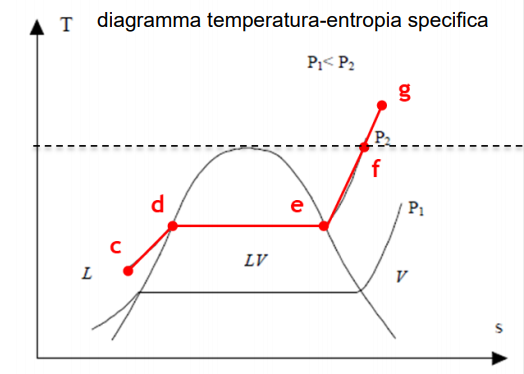
\includegraphics[height=6cm]{../L04/img9.PNG}
\end{center}
Il tipo di diagramma utilizzato varia a seconda dello scopo che si vuole raggiungere, ce ne sono anche molti altri, per esempio quello $P-h$ e quello $h-s$.
\subsection{Proprietà termodinamiche dei sistemi eterogenei}
\subsubsection{Entalpia di transizione di fase}
\[
    h_{solido} < h_{liquido} < h_{vapore}
\]
\begin{itemize}
    \item entalpia di \textbf{liquefazione}: $h_{liquido}-h_{solido} > 0$
    \item entalpia di \textbf{solidificazione}: $h_{lst}= h_{solido}- h_{liquido} < 0$
    \item entalpia di \textbf{evaporazione}: $h_{lvt} = h_{vapore}- h_{liquido} >0$
    \item entalpia di \textbf{condensazione}: $h_{liquido}-h_{vapore} <0$
    \item entalpia di \textbf{sublimazione}: $h_{svt} = h_{vapore}- h_{solido} >0$
    \item entalpia di \textbf{brinamento}: $h_{solido}-h_{vapore} <0$
\end{itemize}
\subsubsection{Titoli}
Le frazioni massiche dei tre stati di aggregazione prendono il nome di \textbf{titolo}:
\begin{itemize}
    \item \textbf{titolo di vapore}: $x_v = \frac{M_v}{M}$
    \item \textbf{titolo di liquido}: $x_l = \frac{M_l}{M}$
    \item \textbf{titolo di solido}: $x_s = \frac{M_s}{M}$
\end{itemize}
Ricordiamo che $x_v + x_l + x_s = 1$ e che una generica \textbf{grandezza estensiva} $e$ può essere espressa come:
\[
    e = (1-x_l-x_v) e_s + x_l e_l + x_v e_v
\]
\subsection{Tabelle termodinamiche}
\subsubsection{Tabella di saturazione in pressione}
E' detta "in pressione" perchè sulla prima colonna sono indicate le \textbf{pressioni}.\newline
La seconda colonna rappresenta delle \textbf{temperature}.\newline
\newline
La prima riga è sempre quella che rappresenta il \textbf{punto triplo}.\newline
\newline
Ogni coppia di valori Pressione-Temperatura presente in tabella segue la \textbf{curva di saturazione liquido-vapore} proiettata su un diagramma $P-T$.\newline
\newline
Per ogni coppia $P-T$ specificato in tabella sono indicati i seguenti valori:
\begin{itemize}
    \item \textbf{volume specifico} (terza, quarta, quinta colonna)
    \item \textbf{entalpia specifica} (sesta, settima, ottava colonna)
    \item \textbf{entropia specifica} (nona, decima, undicesima colonna)
\end{itemize}
Per ognuno di questi valori viene indicato il valore per \textbf{liquido saturo}, per \textbf{vapore saturo} e la differenza fra questi ultimi due.
\begin{center}
    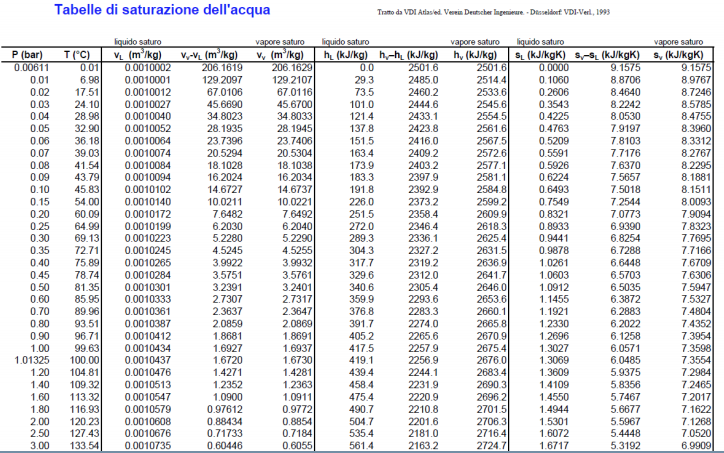
\includegraphics[height=7cm]{../L04/img10.PNG}
\end{center}
\subsubsection{Tabella di saturazione in temperatura}
E' detta "in temperatura" perchè sulla prima colonna sono indicate le \textbf{temperature}.\newline
La seconda colonna rappresenta delle \textbf{pressioni}.\newline
\newline
Il contenuto della tabella è il medesimo della tabella precedente, solo che il riferimento è basato sulla temperatura (sono in ordine di temperatura) e non sulla pressione.
\begin{center}
    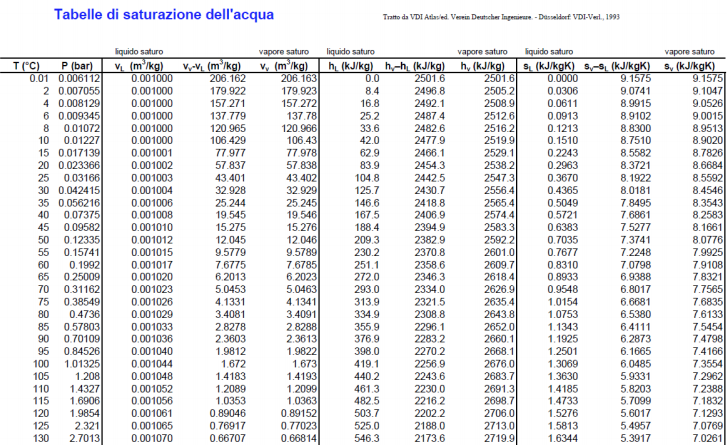
\includegraphics[height=7cm]{../L04/img11.PNG}
\end{center}
\subsubsection{Tabella del vapore surriscaldato}
Questa tabella mostra le pressioni sulle righe e le temperature sulle colonne, per un sistema monofase, in cui $P$ e $T$ descrivono uno stato di equilibrio.\newline
\newline
Per ogni riga di pressione, è mostrata la \textbf{temperatura} $T_s$ di \textbf{saturazione} a tale pressione.\newline
\newline
Per ogni coppia temperatura - pressione che andiamo a cercare  troviamo i valori di \textbf{volume specifico}, \textbf{entalpia specifica}, \textbf{entropia specifica}.\newline
\newline
La zona evidenziata in giallo, senza valori, rappresentano i valori oltre la curva limite, cioè la zona di liquido sottoraffreddato, dove $T_s > T$.
\begin{center}
    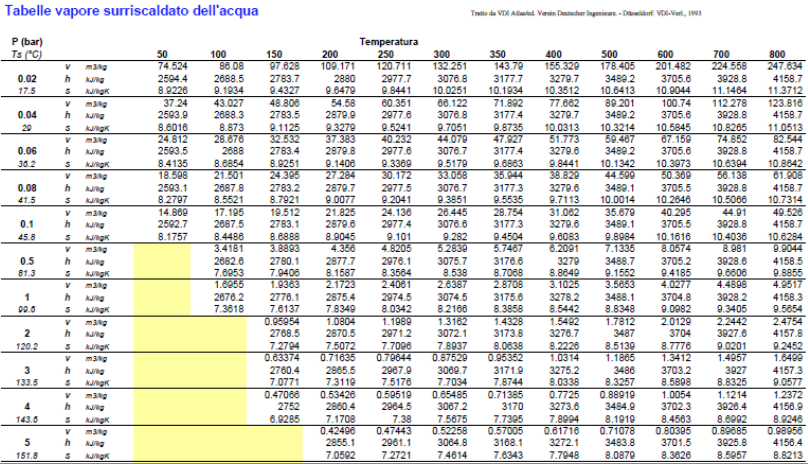
\includegraphics[height=7cm]{../L04/img12.PNG}
\end{center}
\subsubsection{Interpolazione lineare}
Siccome non è possibile creare tabelle con ogni possibile valore, per tutti quei casi in cui non si trova una corrispondenza precisa nella tabella, si usa lì \textbf{interpolazione lineare}
\[
    Y = Y_A + \frac{Y_B - Y_A}{X_B - X_A}(X - X_A)
\]
$Y$: grandezza che si vuole ricavare.\newline
$X$: grandezza conosciuta.\newline
$A,B$: stati di riferimento (presenti in tabella) con $X_A < X < X_B$.
\subsubsection{interpolazione bilineare}
Nel caso in cui più di una grandezza non corrisponda a nessun valore preciso della tabella usiamo la formula di \textbf{interpolazione bilineare}
\[
    Y = Y_A + \frac{Y_B - Y_A}{X_B - X_A}(X - X_A)
\]
\[
    Y_A = Y_{A1} + \frac{Y_{A2}- Y_{A1}}{X_{A2}- X_{A1}} (X_A - X_{A1})
\]
\[
    Y_B = Y_{B1} + \frac{Y_{B2}- Y_{B1}}{X_{B2}- X_{B1}} (X_B - X_{B1})
\]
\subsubsection{Formule per l'acqua sottoraffreddata}
Vediamo come calcolare tutti quei valori per cui non esistono tabelle, per esempio i valori per un liquido sottoraffreddato.\newline
\newline
\textbf{Modello di liquido incomprimibile ideale}\newline
Per un liquido incomprimibile ideale abbiamo $c_P = c(T), \beta = 0, K_T = 0$ e
\[
    dh = c(T) dT + v dP
\]
\[
    ds = c(T) \frac{dT}{T}
\]
che sono forme differenziali e per poterle integrare devo conoscere la funzione $c(T)$, che però non conosciamo. L'ipotesi che quindi facciamo è quella di liquido incomprimibile perfetto, cioè con $c$ costante.\newline
\newline
\textbf{Modello di liquido incomprimibile perfetto}\newline
Per un liquido incomprimibile perfetto abbiamo $c = costaten$ e quindi possiamo integrare le formule viste precedentemente e otteniamo
\[
    \Delta h = c\Delta T + v \Delta P
\]
\[
    \Delta s = c ln \frac{T_2}{T_1}
\]
Dalla prima di queste due formule posso scrivere che
\[
    h - h_{ref} = c(T-T_{ref}) + v (P-P_{ref})
\]
dove col pedice "ref" si intendono valori che troviamo in tabella per liquidi saturi.\newline
\newline
Possiamo ora procedere in due maniere: fissando la temperatura (corretto) o fissando la pressione (sbagliato).\newline
\newline
\textbf{Approccio a temperatura costante}:
\begin{center}
    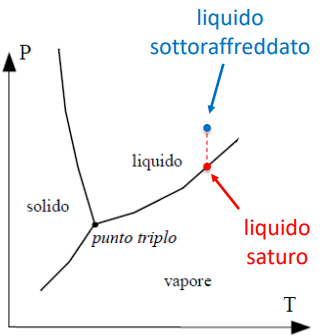
\includegraphics[height=5cm]{../L04/img13.PNG}
\end{center}
La situazione è questa: stiamo cercando di calcolare il punto azzurro di "liquido sottoraffreddato" usando le tabelle di liquido saturo che ci permettono di individuare il punto rosso di "liquido saturo" alla medesima temperatura.
\newline
sostituiamo i valori con pedice "ref" dell'equazione precedentemente trovata
\[
    h - h_{ref} = c(T-T_{ref}) + v (P-P_{ref})
\]
con i valori che troviamo con la tabella di liquido saturo eccetto per la temperatura che teniamo fissa:
\[
    h(P,T) - h_{ls}(P_{sat}(T)) = c(T - T) + v (P - P_{sat}(T))
\]
\[
    h(P,T) = h_{ls} (P_{sat}(T)) + v (P-P_{sat}(T))
\]
inoltre per $v$ si può usare il valore del liquido saturo fornito dalla tabella $v = v_{ls}(P_{sat}(T))$.\newline
\newline
\textbf{Approccio a pressione costante}:\newline
\textbf{N.B. non usare questo approccio!}
\begin{center}
    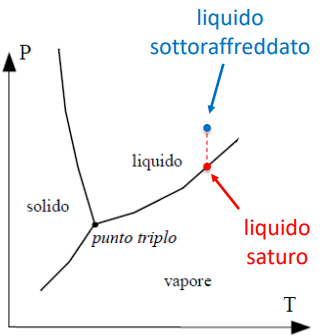
\includegraphics[height=5cm]{../L04/img13.PNG}
\end{center}
La situazione è questa: stiamo cercando di calcolare il punto verde di "liquido sottoraffreddato" usando le tabelle di liquido saturo che ci permettono di individuare il punto rosso di "liquido saturo" alla medesima pressione.\newline
Se seguiamo il medesimo procedimento di prima ma con pressione fissa, otteniamo:
\[
    h(P,T) - h_{ls}(T_{sat}(P)) = c (T-T_{sat}(P)) + v(P-P)
\]
\[
    h(P,T) = h_{ls}(P_{sat} (T)) + c (T-T_{sat}(P))
\]
che non è valido perchè in genere $c \neq costante$.\newline
Cosa fare se si conosce $P$ e non $T$? (TODO, vedi esercizio ES 3.1.6)\newline
\newline
\textbf{Caso nel quale si conosce (P,h) e si vuole conoscere T}\newline
\[
    h(P,T) = h_{ls}(P_{sat}(T)) + v(P-P_{sat}(T))
\]
in cui solitamente $v (P-P_{sat}(T))$ è solitamente trascurabile, e dunque si interpola in tabella di saturazione la temperatura per la quale $h_{ls}(T) = h$.\newline
\newline
\textbf{Caso nel quale si conosce (P,s) e si vuole conoscere T}\newline
Approccio simile a quello precedente.
\subsection{Relazioni semplificate vicino al punto triplo per l'acqua}
In assenza di tabelle, si possono usare le seguenti relazioni semplificate che rimandono valide in prossimità \textbf{punto triplo} per lo stato solido, lo stato liquido e lo stato vapore.
\begin{center}
    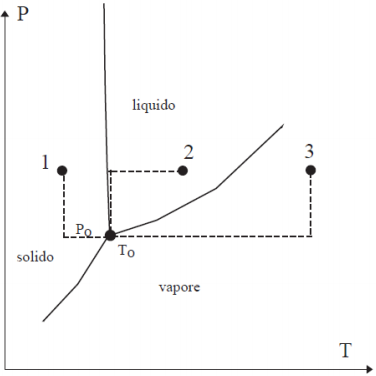
\includegraphics[height=5cm]{../L04/img15.PNG}
\end{center}
\subsubsection{Stato solido}
\[
    h(P,T) = h_0 + h_{lst} + c_s(T-T_0) + v_s(P-P_0)
\]
\[
    s(P,T) = s_0 +s_{lst} + c_s ln \frac{T}{T_0} = s_0 + \frac{h_{lst}}{T_0} + c_s ln \frac{T}{T_0}
\]
con \newline
$P_0, T_0$: pressione e temperatura del punto triplo ($P_0 = 0,00611 bar ; T_0 = 0.01 C^o$)\newline
$h_0$: entalpia di riferimento al punto triplo in fase liquida ($h_0 = 0 kJ/kg$)\newline
$s_0$: entropia di riferimento al punto triplo in fase liquida ($s_0 = 0kJ/kgK$)\newline
$h_{lst}$: entalpia di solidificazione al punto triplo ($h_{lst} = -333 kJ/kg$)\newline
$c_s$: calore specifico del ghiaccio ($c_s = 2093 J/kgK$)\newline
$v_s$: volume specifico del ghiaccio ($v_s = 0.00109 m^3/kg$)\newline
Possiamo approssimare $T_{sat, L-S}(P) = T_0$.
\subsubsection{Stato liquido}
(USARE LE TABELLE)
\[
    h(P,T) = h_0 + c_{l}(T-T_0) + v_l (P-P_0)
\]
\[
    s(P,T) = s_0 + c_l ln \frac{T}{T_0}
\]
con \newline
$P_0, T_0$: pressione e temperatura del punto triplo ($P_0 = 0,00611 bar ; T_0 = 0.01 C^o$)\newline
$h_0$: entalpia di riferimento al punto triplo in fase liquida ($h_0 = 0 kJ/kg$)\newline
$s_0$: entropia di riferimento al punto triplo in fase liquida ($s_0 = 0kJ/kgK$)\newline
$c_{l}$: calore specifico dell'acqua liquida ($c_l = 4186 J/kgK$)\newline
$v_{l}$: volume specifico dell'acqua liquida ($v_l = 0,001 m^s/kg$)
\subsubsection{Stato vapore}
(USARE LE TABELLE)
\[
    h(P,T) = h_0 + h_{lvt} + c_p (T-T_0)
\]
\[
    s(P,T) = s_0 + s_{lvt} + c_p ln \frac{T}{T_0} - R^* ln \frac{P}{P_0} = s_0 + \frac{h_{lvt}}{T_0} c_P ln \frac{T}{T_0}- R^* ln \frac{P}{P_0}
\]
con \newline
$P_0, T_0$: pressione e temperatura del punto triplo ($P_0 = 0,00611 bar ; T_0 = 0.01 C^o$)\newline
$h_0$: entalpia di riferimento al punto triplo in fase liquida ($h_0 = 0 kJ/kg$)\newline
$s_0$: entropia di riferimento al punto triplo in fase liquida ($s_0 = 0kJ/kgK$)\newline
$h_{lvt}$: entalpia di evaporazione al punto triplo ($h_{lvt} = 2501.6 kJ/kg$)\newline
$c_P$: calore specifico a pressione costante dell'acqua vapore ($c_P = 2009 J/kgK$)
    \newpage
    \url{../pdf/Lezioni/L05-Macchine termodinamiche-con-annotazioni.pdf}
    \section{L05-Macchine termodinamiche}
\subsection{Macchina termodinamica}
Per rappresentare \textbf{macchine termodinamiche} utiliziamo solitamente questa struttura:
\begin{center}
    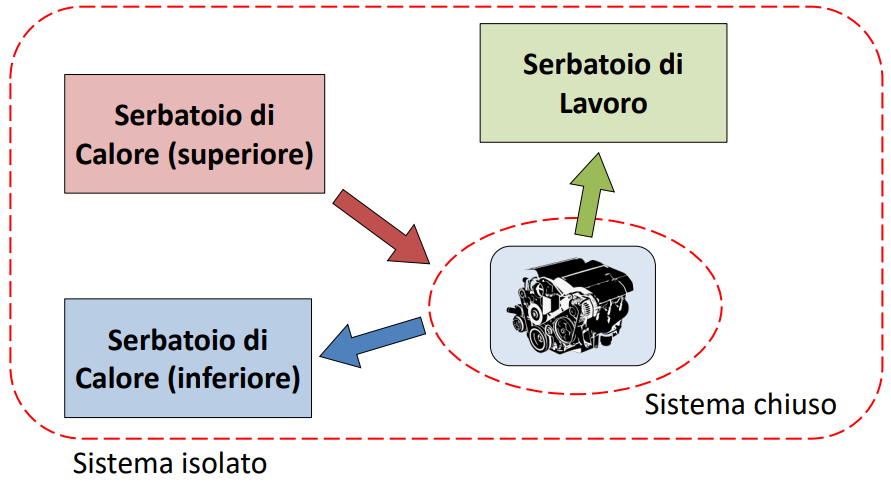
\includegraphics[height=5cm]{../L05/img1.PNG}
\end{center}
La \textbf{macchina termodinamica} è un sistema termodinamico \textbf{composto} e \textbf{isolato}, che, nella sua forma più semplice, è realizzato da:
\begin{itemize}
    \item due serbatoi di calore, uno superiore e uno inferiore;
    \item un serbatoio di lavoro;
    \item una macchina ciclica, che è in grado di produrre od assorbire con continuità lavoro interagendo con il serbatoio di lavoro ed i serbatoi di calore.
\end{itemize}
\subsubsection{Serbatoio di calore}
Il \textbf{serbatoio di calore} è un sistema termodinamico che scambia \textbf{solo calore} con l'esterno senza alterare il suo stato termodinamico (cioè la temperatura e la pressione del serbatoio rimangono costanti, tutto ciò che è al suo interno rimane costante, il suo stato non cambia); gli scambi avvengono con trasformazioni quasi-statiche (\textbf{internamente reversibili}).\newline
\newline
Questa definizione di serbatoio è sinonimo di un sistema \textbf{a massa infinita}: se la massa di un sistema $A$ è enormemente maggiore della massa di un sistema $B$, durante un interazione fra $A$ e $B$, $A$ sembrerà rimanere invariata, poichè tutte le trasformazioni e tutte le grandezze sono legate in proporzione alla massa.\newline
\newline
Un tipico esempio di serbatoio di calore e l'atmosfera terrestre.
\subsubsection{Serbatoio di lavoro}
Il \textbf{serbatoio di lavoro} è un sistema termodinamico che scambia \textbf{solo lavoro} con l'esterno senza alterare il suo stato termodinamico; gli scambi avvengono con trasformazioni quasi-statiche (\textbf{internamente reversibili}).\newline
\newline
Un tipico esempio di serbatoio di lavoro è la rete elettrica.
\subsubsection{Macchina motrice}
Per \textbf{macchina ciclica} si intendono macchine che compiono trasformazioni con stato finale e stato iniziale identici e ripetono $n$ volte tale ciclo.\newline
\newline
Esistono due schemi principali di macchine cicliche: quelle motrici e quelle operatrici. Vediamo la macchina motrice. \newline
\newline
Il \textbf{serbatoio superiore} è a \textbf{temperatura calda} $T_C$ e prende il nome di \textbf{camera di combustione}.\newline
Il serbatoio di calore a $T_C$ e la macchina ciclica, producono un lavoro verso il serbatoio di lavoro e devono rilasciare calore verso un \textbf{serbatoio inferiore} a \textbf{temperatura fredda} $T_F$ che tipicamente è l'\textbf{ambiente}.
\begin{center}
    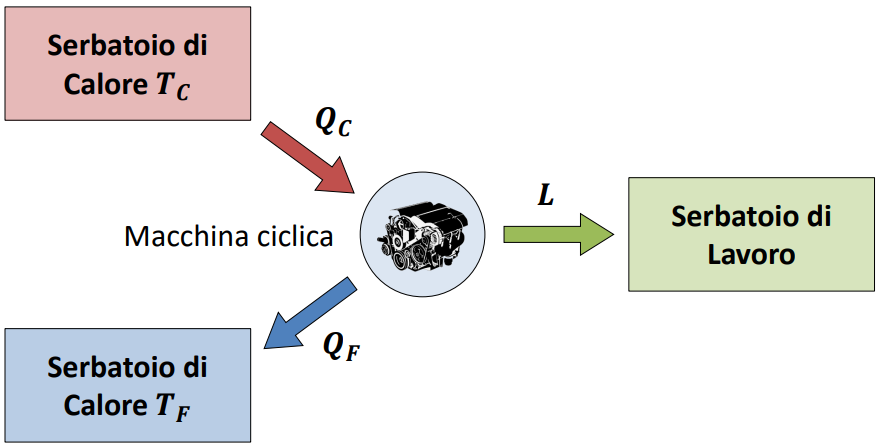
\includegraphics[height=5cm]{../L05/img2.PNG}
\end{center}
Vediamo la macchina motrice da un punto di vista analitico.\newline
Dalle equazioni di bilancio otteniamo:
\[
    \begin{cases}
        \Delta U_Z = 0\\ \Delta S_Z = S_{irr}
    \end{cases} \;\;\;\;\;\;\;\;\;\;\;\;\;\;\; \begin{cases}
        \Delta U_C + \Delta U_F + \Delta U_{SL} + \Delta U_M = 0 \\
        \Delta S_C + \Delta S_F + \Delta S_{SL} + \Delta S_M = S_{irr}
    \end{cases}
\]
Osservando i singoli sottosistemi otteniamo:
\[
    \begin{cases}
        \Delta U_C = Q_C^\leftarrow \\ \Delta S_C = \frac{Q_C^\leftarrow }{T_C}
    \end{cases} \;\;\;\;\; \begin{cases}
        \Delta U_F = Q_F^\leftarrow \\ \Delta S_F = \frac{Q_F^\leftarrow}{T_F}
    \end{cases} \;\;\;\;\; \begin{cases}
        \Delta U_{SL} = - L_{SL}^\rightarrow \\ \Delta S_{SL} = 0
    \end{cases} \;\;\;\;\; \begin{cases}
        \Delta U_M = 0\\ \Delta S_M = 0
    \end{cases}
\]
Per cui deriviamo che
\[
    \begin{cases}
        Q_C^\leftarrow  + Q_F^\leftarrow  - L_{SL}^\rightarrow  = 0\\
        \frac{Q_C^\leftarrow}{T_C} + \frac{Q_F^\leftarrow}{T_F} = S_{irr}
    \end{cases} \;\;\;\;\;\;\;\;\;\; \begin{cases}
        -Q_C + Q_F + L = 0\\
        -\frac{Q_C}{T_C} + \frac{Q_F}{T_F} = S_{irr}
    \end{cases}
\]
\textbf{Rendimento}:\newline
Da queste equazioni ricaviamo che il lavoro è massimo quando il processo è \textbf{reversibile}, per cui il \textbf{rendimento} è
\[
    \eta = \frac{\text{EFFETTO UTILE}}{\text{SPESA}}
\]
La definizione di rendimento si traduce in formule per la macchina motrice così:
\[
    \eta = \frac{L}{Q_C} = 1- \frac{T_F}{T_C} - \frac{T_F}{Q_C} S_{irr} \;\;\;\;\;\;\;\;\;\;\eta_{reversibile} = 1 - \frac{T_F}{T_C}
\]
dove $\eta_{reversibile}$ viene utilizzato per calcolare il rendimento massimo che si può avere.\newline
Queste formule sono valide per serbatoi di calore a temperatura costante, nel momento in cui questa condizione viene meno, non possiamo più usarle, però possiamo sempre usare la definizione di rendimento (effetto utile/ spesa).
\subsubsection{Macchina operatrice}
La \textbf{macchina operatrice} ha un meccanismo opposto alla macchina motrice: usa del lavoro dal \textbf{serbatoio di lavoro} per assorbire calore da un \textbf{serbatoio freddo}, a causa dell'utilizzo di questo lavoro c'è bisogno di rilasciare del calore in un \textbf{serbatoio caldo}.
\begin{center}
    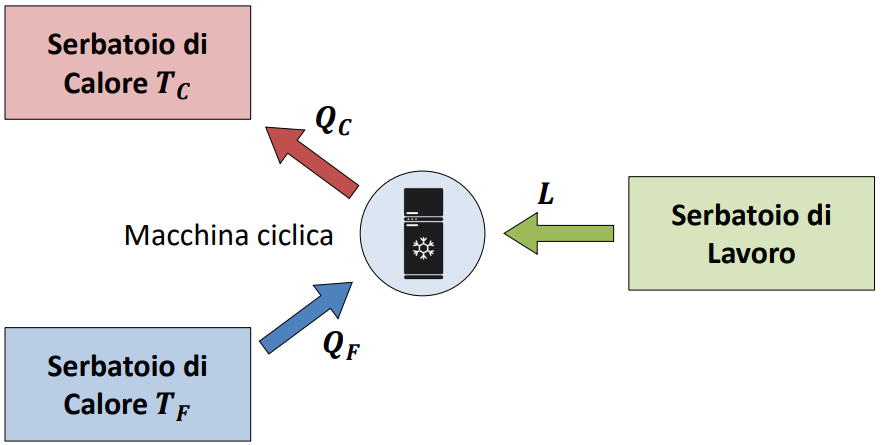
\includegraphics[height=5cm]{../L05/img3.PNG}
\end{center}
Vediamo la macchina operatrice da un punto di vista analitico.\newline
Dalle equazioni di bilancio otteniamo:
\[
    \begin{cases}
        \Delta U_Z = 0\\ \Delta S_Z = S_{irr}
    \end{cases} \;\;\;\;\;\;\;\;\;\;\;\;\;\;\; \begin{cases}
        \Delta U_C + \Delta U_F + \Delta U_{SL} + \Delta U_M = 0 \\
        \Delta S_C + \Delta S_F + \Delta S_{SL} + \Delta S_M = S_{irr}
    \end{cases}
\]
Osservando i singoli sottosistemi otteniamo:
\[
    \begin{cases}
        \Delta U_C = Q_C^\leftarrow \\ \Delta S_C = \frac{Q_C^\leftarrow }{T_C}
    \end{cases} \;\;\;\;\; \begin{cases}
        \Delta U_F = Q_F^\leftarrow \\ \Delta S_F = \frac{Q_F^\leftarrow}{T_F}
    \end{cases} \;\;\;\;\; \begin{cases}
        \Delta U_{SL} = - L_{SL}^\rightarrow \\ \Delta S_{SL} = 0
    \end{cases} \;\;\;\;\; \begin{cases}
        \Delta U_M = 0\\ \Delta S_M = 0
    \end{cases}
\]
Per cui deriviamo che
\[
    \begin{cases}
        Q_C^\leftarrow  + Q_F^\leftarrow  - L_{SL}^\rightarrow  = 0\\
        \frac{Q_C^\leftarrow}{T_C} + \frac{Q_F^\leftarrow}{T_F} = S_{irr}
    \end{cases} \;\;\;\;\;\;\;\;\;\; \begin{cases}
        Q_C - Q_F - L = 0\\
        \frac{Q_C}{T_C} - \frac{Q_F}{T_F} = S_{irr}
    \end{cases}
\]
\textbf{L'unica cosa che cambia rispetto alla macchina motrice sono i segni}.\newline
\newline
\textbf{Efficienza o COP (coefficient of performance)}:\newline
Il lavoro è minimo quando il processo è \textbf{reversibile}, per cui l'\textbf{efficienza} è
\[
    \epsilon = \frac{\text{EFFETTO UTILE}}{\text{SPESA}}
\]
Vediamo ora la formula dell'efficienza nei casi particolari di macchina operatrice \textbf{frigorifera} e \textbf{pompa di calore}:\newline
\textbf{Macchina frigorifera}:
\[
    \epsilon_F = \frac{Q_F}{L} = \frac{T_F}{T_C - T_F + \frac{T_CT_FS_{irr}}{Q_F}} \;\;\;\;\;\;\;\;\;\; \epsilon_{F,reversibile} = \frac{T_F}{T_C-T_F}
\]
dove $\epsilon_{reversibile}$ viene utilizzato per calcolare l'efficienza massima che si può avere.\newline
\textbf{Pompa di calore}:
\[
    \epsilon_P = \frac{Q_C}{L} = \frac{T_C}{T_C - T_F + \frac{T_CT_FS_{irr}}{Q_C}} \;\;\;\;\;\;\;\;\;\; \epsilon_{P,reversibile} = \frac{T_C}{T_C-T_F}
\]
dove $\epsilon_{reversibile}$ viene utilizzato per calcolare l'efficienza massima che si può avere.\newline
\newline
Queste formule sono valide per serbatoi di calore a temperatura costante, nel momento in cui questa condizione viene meno, non possiamo più usarle, però possiamo sempre usare la definizione di efficienza (effetto utile/ spesa).
\newline
\newline
C'è un legame fra l'efficienza della macchina frigorifera e l'efficienza della pompa di calore:
\[
    \epsilon_P = \frac{Q_C}{L} = \frac{Q_F+L}{L} = \epsilon_F + 1
\]
\subsubsection{Macchina motrice con serbatoio caldo a massa finita}
Fino ad ora abbiamo analizzato il comportamento di macchine termodinamiche con serbatoi a massa infinita e quindi temperatura costatne. Vediamo ora il ragionamento che sta sotto l'analisi di macchine motrici con serbatoio caldp a \textbf{massa finita}.\newline
\newline
Per semplificare la trattazione analiziamo \textbf{Macchina motrice con serbatoio caldo a massa finita contenente liquido incomprimibile perfetto} (vediamo il caso con liquido incomprimibile perfetto, ma questo dettaglio ha un impatto irrilevante sulla trattazione, lo usiamo sol oper semplicità di esposizione, si può rieseguire il ragionamento anche con gas perfetti e altro ancora\dots).\newline
\newline
Dalle equazioni di bilancio otteniamo:
\[
    \begin{cases}
        \Delta U_Z = 0\\ \Delta S_Z = S_{irr}
    \end{cases} \;\;\;\;\;\;\;\;\;\;\;\;\;\;\; \begin{cases}
        \Delta U_C + \Delta U_F + \Delta U_{SL} + \Delta U_M = 0 \\
        \Delta S_C + \Delta S_F + \Delta S_{SL} + \Delta S_M = S_{irr}
    \end{cases}
\]
Nel serbatoio a caldo la temperatura iniziale è maggiore di quella finale ($T_1 > T_2$), l'altro serbatoio rimane invece a temperatura costante, per cui:
\[ 
    \begin{cases}
        \Delta U_{C,12} = Mc(T_2 -T_1)\\ \Delta S_{C,12} = Mcln \frac{T_2}{T_1}
    \end{cases}\;\;\;\;\; \begin{cases}
        \Delta U_F = Q_F^\leftarrow \\ \Delta S_F = \frac{Q_F^\leftarrow}{T_F}
    \end{cases} \;\;\;\;\; \begin{cases}
        \Delta U_{SL} = - L_{SL}^\rightarrow \\ \Delta S_{SL} = 0
    \end{cases} \;\;\;\;\; \begin{cases}
        \Delta U_M = 0\\ \Delta S_M = 0
    \end{cases}
\]
Per cui deriviamo che
\[
    \begin{cases}
        Mc(T_2-T_1) + Q_f^\leftarrow - L_{SL}^\rightarrow  = 0\\
        Mc ln \frac{T_2}{T_1} + \frac{Q_F^\leftarrow}{T_F} = S_{irr}
    \end{cases} \;\;\;\;\;\;\;\;\;\; \begin{cases}
        Mc(T_2-T_1) + Q_F + L = 0\\ Mc ln \frac{T_2}{T_1} + \frac{Q_F}{T_F} = S_{irr}
    \end{cases}
\]
\textbf{Caso reversibile} $S_{irr} = 0$:
$Q_C^\leftarrow =  Mc(T_2-T_1)$ negativo uscente; \newline
$Q_C =  Mc(T_2-T_1)$ valore assoluto; \newline
\newline
$Q_F^\leftarrow  = - Mc T_F ln \frac{T_2}{T_1} = Mc T_F ln \frac{T_1}{T_2}$ positivo entrante;\newline
$Q_F = Mc T_F ln \frac{T_1}{T_2}$ valore assoluto.\newline
\newline
$L^\rightarrow  = Q_C^\leftarrow  + Q_F^\leftarrow  = Mc(T_2 -T_1) + Mc T_F ln \frac{T_1}{T_2}$ negativo entrante;\newline
$L = Q_C- Q_F = Mc (T_1-T_2) - McT_F ln \frac{T_1}{T_2}$ valore assoluto.\newline
\newline
Rendimento $\eta = \frac{L}{Q_C}$ e $\eta_{rev} = \frac{L_{rev}}{Q_C}$.\newline
\newline
\textbf{Rendimento di secondo principio per la macchina motrice}:
\[
    \eta_{II} = \frac{\eta}{\eta_{rev}} = \frac{L}{L_{rev}}
\]
\textbf{Rendimento di secondo principio per la macchina operatrice}:
\[
    \eta_{II} = \frac{\epsilon}{\epsilon_{rev}} = \frac{L_{rev}}{L}
\]
    \newpage
    \url{../pdf/Lezioni/L06-Sistemi aperti-con-annotazioni.pdf}
    \section{L01-Sistemi aperti}
    \newpage
    \url{../pdf/Lezioni/L07-Cicli a gas-con-annotazioni.pdf}
    \section{L07-Cicli a gas}
\subsection{Cicli termodinamici a gas}
Vedremo molte formule e molti passaggi che però non è essenziale imparare benissimo. Queste formule semplificate saranno solo \textbf{valide per cicli ideali}, quindi nel momento in cui si analizza un ciclo reale non valgono più. Ciò che sarà applicabile anche nei casi reali sono le definizioni che mostreremo.\newline
\newline
Nei cicli termodinamici a gas faremo sempre l'\textbf{ipotesi} semplificativa \textbf{di gas perfetti} (anche se non è sempre propriamente valido).\newline
\newline
Esistono numerosi cicli:
\begin{itemize}
    \item Ciclo di Carnot (ciclo puramente teorico, irrealizzabile nella realtà);
    \item Ciclo Joule-Brayton (tipico degli aerei);
    \item Ciclo Otto (tipico ciclo che utilizza benzina, quindi automobili, tosaerba, etc);
    \item Ciclo Diesel (tipico per le applicazioni a potenze elevate);
    \item Ciclo Stirling (importante a livello storico);
    \item Ciclo Ericsson;
\end{itemize}
\subsubsection{Proprietà dei cicli simmetrici}
Un ciclo termodinamico è tipicamente rappresentato da $4$ \textbf{politropiche}, uguali a due a due, per cui prende il nome di ciclo \textbf{simmetrico}. Non sempre questa ipotesi di simmetria è presente.
\begin{center}
    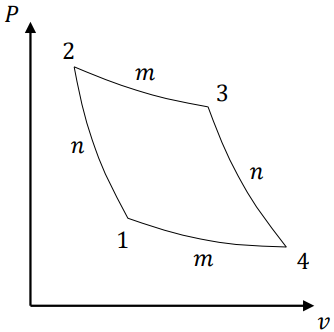
\includegraphics[height=3cm]{../L07/img1.PNG}
\end{center}
Nel caso di \textbf{ciclo ideale} (politropiche senza irreversibilità, cioè trasformazioni internamente reversibili) e ipotesi di \textbf{gas ideale}:
\[
    \begin{matrix}
        v_1v_3 = v_2v_4\\
        P_1P_3 = P_2P_4\\
        T_1T_3 = T_2T_4
    \end{matrix}
\]
(Queste formule derivano dalla scrittura delle politropiche di ogni trasformazione e utilizzando l'equazione di stato dei gas ideali e facendo alcuni passaggi e calcoli).\newline
\newline
La maggior parte dei cicli che andremo a vedere sono principalmente utilizzati per macchina motrici (che producono lavoro). Più avanti vedremo esempi di cicli inversi che verranno usati per macchine operatrici.\newline
\newline
Fino ad ora per le macchine termodinamiche abbiamo parlato dei serbatori di calore a temperatura calda e fredda e del serbatoio di lavoro, ora ci focaliziamo sulla macchina ciclica che opera su questi serbatoi.\newline
\newline
Il termine $S_{irr}$ che abbiamo nel bilancio entropico può essere scomposto in $S_{irr,est}$, cioè le irreveribilità esterne (legate ai serbatoi e agli scambi), e $S_{irr, int}$, cioè le irreversibilità interne della macchina ciclica (irreversibilità delle trasformazioni). Nel caso ideale non avremo irreversibilità esterne, quindi nessuna irreversibilità nei serbatoi e negli scambi con la macchina ciclica. Se le tr
\subsection{Ciclo di Carnot}
Il \textbf{ciclo di Carnot} è un \textbf{ciclo teorico} composto da $4$ trasformazioni tutte internamente reversibili e l'unica combinazioni di trasformazioni politropiche che soddisfano queste richieste sono \textbf{due isoentropiche e due isoterme}.
\begin{center}
    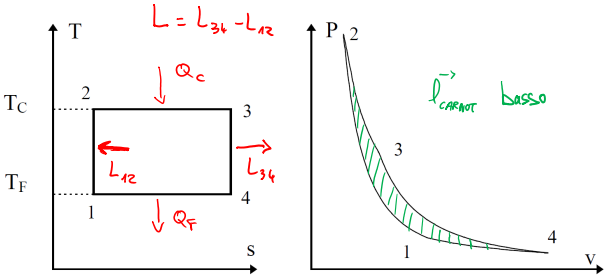
\includegraphics[height=4cm]{../L07/img2.PNG}
\end{center}
In (2-3) avviene lo scambio di calore con il serbatoio di calore superiore, in (4-1) avviene lo scambio di calore con il serbatoio di calore inferiore. Queste due sono le trasformazioni isoterme. Invece lungo le isoentropiche (1-2) e (3-4) non abbiamo scambi di calore, ma solo di lavoro, le isoentropiche sono adiabatiche reversibili. Il lavoro totale uscente dal ciclo (il lavoro prodotto) sarà calcolabile come $L = L_{34} - L_{12}$. \newline
\newline
Questo ciclo rappresenta il ciclo ideale che si cerca di ottenere per una macchina per avere il rendimento massimo.\newline
\newline
Guardando il diagramma P-V vediamo che l'area interna al ciclo (che rappresenta il lavoro specifico) è molto ridotto. Il lavoro specifico del ciclo di Carnot è molto basso, nonostante il rendimento sia massimo. Questo vuol dire che per avere una certa potenza dobbiamo avere un impianto di dimensioni notevoli.\newline
\newline
\subsubsection{Rendimento del ciclo}:
\[
    \eta = \frac{L}{Q_C} = 1-\frac{Q_F}{Q_C} = 1- \frac{T_1}{T_3}    
\]
\ \newline
\newline
\textbf{Possibili fonti di irreversibilità per una macchina termodinamica}:
\begin{itemize}
    \item \textbf{Irreversibilità esterna ($T_{min} > T_F$ e $T_{max} < T_C$)}:\newline
    Ricordiamo che $T_1 = T_4 = T_{min}$ e $T_2 = T_3 = T_{max}$.
    \begin{center}
        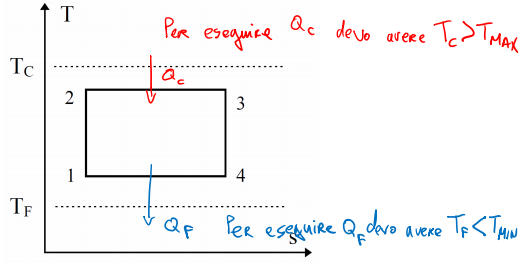
\includegraphics[height=3cm]{../L07/img3.PNG}
    \end{center}
    Tipico caso di irreversibiltà esterna è il fatto che le temperature dei serbatoi non coincidano con le temperature delle trasformazioni.
    \[
        \eta_{rev} = 1-\frac{T_F}{T_C} > \eta_{ciclo} = 1- \frac{T_1}{T_3} = 1- \frac{T_{min}}{T_{max}}
    \]
    Bilancio entropico su tutta la macchina termica (reale):
    \[
        -\frac{Q_C}{T_C} + \frac{Q_F}{T_F} = S_{irr}
    \]
    Per il ciclo di Carnot vale:
    \[
        \frac{Q_C}{T_3} = \frac{Q_F}{T_1} = \Delta S
    \]
    Che risolta rispettoa $Q_F$:
    \[
        Q_C\left(\frac{1}{T_F} \frac{T_1}{T_3} - \frac{1}{T_C}\right) = S_{irr}
    \]
    \[
        Q_C \left(\frac{T_C T_1 - T_F T_3}{T_3T_CT_F}\right) = S_{irr, est} > 0
    \]
    \item \textbf{Irreversibilità interna ($s_1 > s_2$ e $s_3 < s_4$)}:
    \item \begin{center}
        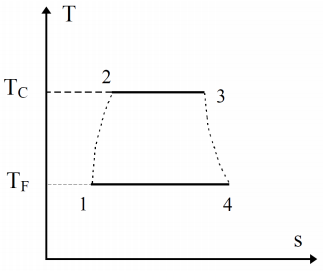
\includegraphics[height=3cm]{../L07/img4.PNG}
    \end{center}
    In questo caso non abbiamo più isoentropiche, ma trasformazioni reali, per cui si ha un incremento di entropia.\newline
    Bilancio entropico su tutta la macchina termica (reale):
    \[
        - \frac{Q_C}{T_C} + \frac{Q_F}{T_F} = S_{irr}
    \]
    per cui:
    \[
        \frac{Q_C}{T_C} = S_3 - S_2
    \]
    \[
        \frac{Q_F}{T_F} = S_4 - S_1
    \]
    e sostitendo:
    \[
        S_2-S_3 +S_4 -S_1 = S_{irr, int} > 0
    \]
\end{itemize}
Nel caso in cui si abbiano entrambe le irreversibilità, le due componenti si sommano.
\subsection{Ciclo di Joule-Bryton}
\textbf{Caso simmetrico costituitio da due isoentropiche e due isobare}:\newline
Abbiamo detto che il ciclo di Carnot è ideale, per cui non ha applicazioni reali interessanti. Una miglioria che si può fare è quella di considerare trasdormazioni isobare per lo scambio termico. Così facendo si ha un forte incremento della potenza prodotta (area interna al ciclo nel grafico P-V):
\begin{center}
    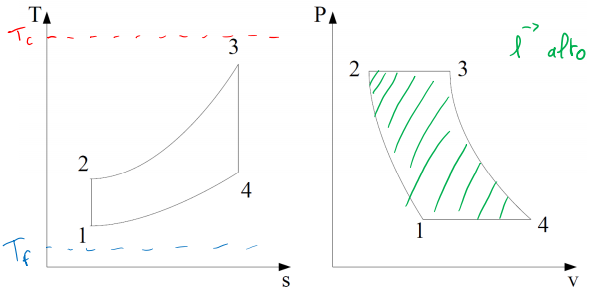
\includegraphics[height=4cm]{../L07/img5.PNG}
\end{center}
Struttura della macchina ciclica per il ciclo di Brayton:
\begin{center}
    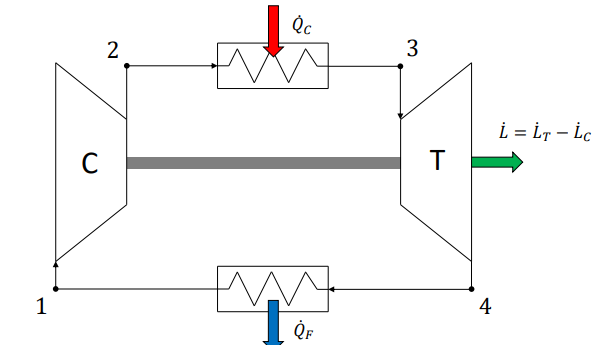
\includegraphics[height=5cm]{../L07/img6.PNG}
\end{center}
dove \newline
$C$: è un compressore che esegue la prima isoentropica;\newline
In alto: uno scambiatore di calore che fa il suo scambio in maniera isobara;\newline
$T$: turbina a gas che esegue la seconda isoentropica;\newline
La barra grigia in centro: mostra che c'è un collegamento fra turbina e compressore, o meglio che turbina e compressore sono sullo stesso asse di rotazione e quindi c'è una trasmissione diretta di potenza fra la turbina e il compressore (una parte di lavoro generata dalla turbina è utilizzata per alimentare il compressore);\newline
In basso: un'altro scambiatore di calore isobaro.\newline
\newline
\subsubsection{Rendimento del ciclo J-B (gas perfetto, ciclo ideale simmetrico)}
Con l’ipotesi di gas perfetto, le equazioni di bilancio energetico per i due serbatoi
di calore sono:
\[
        \dot{Q}_C = \dot{m} (h_3-h_2) \;\;\;\;\;\;\;\;\;\; \dot{Q}_F = \dot{m}(h_4 -h_1)
\]
che con l'ipotesi dei gas perfetti diventa:
\[
    \dot{Q}_C = \dot{m} c_P(T_3-T_2) \;\;\;\;\;\;\;\;\;\; \dot{Q}_F = \dot{m}c_P (T_4-T_1)
\]
Il rendimento termodinamico del ciclo vale:
\[
    \eta_{J-B} = \frac{\dot{L}}{\dot{Q}_C} = 1 - \frac{\dot{Q}_F}{\dot{Q}_C} = 1- \frac{T_4-T_1}{T_3-T_2} = 1- \frac{T_1 \left(\frac{T_4}{T_1} - 1\right)}{T_2 \left(\frac{T_3}{T_2}-1\right)} = 1- \frac{T_1}{T_2}
\]
Inserendo il bilancio di entropia fra 1 e 2 per i gas perfetti:
\[
    \Delta s_{12} = c_P ln \frac{T_2}{T_1}- R^* ln \frac{P_2}{P_1}
\]
\[
    \left(\frac{T_2}{T_1}\right)^{c_P} = \left(\frac{P_2}{P_1}\right)^{R^*}
\]
\[
    \left(\frac{T_2}{T_1}\right) = \left(\frac{P_2}{P_1}\right)^{\frac{R^*}{c_P}} = r_P^{\frac{R^*}{c_P}} = r_P^{\frac{k-1}{k}}
\]
dove $r_P$ è il \textbf{rapporto di compressione} ($\frac{P_2}{P_1}$, che è $\frac{P_{max}}{P_{min}}$) per cui il rendimento è riscrivibile come
\[
    \eta_{J-B} = 1- \frac{1}{r_P^{\frac{k-1}{k}}}
\]
dove $k$ è l'indice della politropica e vale $k = \frac{c_P}{c_V} = costante$.\newline
\newline
Il rendimento del ciclo Joule-Brayton è funzione del solo rapporto di compressione e presenta un minimo (rendimento nullo) quando la pressione $P_2$ tende alla pressione $P_1$ e quindi
\[
    r_{P,min} = 1
\]
mentre ha un valore massimo quando $T_2$ tende a $T_3$, e pertanto
\[
    r_{P,max} = \left(\frac{T_3}{T_1}\right)^{\frac{k}{k-1}}
\]
\subsubsection{Lavoro specifico del ciclo J-B (gas perfetto, ciclo ideale simmetrico)}
Possiamo fare lo stesso ragionamento anche per il lavoro specifico, cioè il lavoro prodotto.\newline
Anche il lavoro specifico utile del ciclo Joule-Brayton ideale è funzione del solo rapporto di compressione
\[
    l = l_T-l_C = c_P (T_3-T_4) - c_P(T_2-T_1)
\]
\[
    l = c_P T_3 \left(1- \frac{T_4}{T_3}\right) - c_P T_1 \left(\frac{T_2}{T_1} - 1\right)
\]
\[
    l = c_P T_3 \left(1- \frac{1}{r_P^{\frac{k-1}{k}}}\right) - c_P T_1 \left(r_P^{\frac{k-1}{k}}-1\right)
\]
Per cui si ha il massimo lavoro specifico in corrispondenza del rapporto di compressione:
\[
    r_{P,opt} = \left(\frac{T_3}{T_1}\right)^{\frac{k}{2(k-1)}} = \sqrt{r_P,max}
\]
Ricordando poi che in una turbina isoentropica
\[
    \frac{T_3}{T_4} = \left(\frac{P_3}{P_4}\right)^{\frac{R^*}{c_P}} = \left(\frac{P_3}{P_4}\right)^\frac{k-1}{k}
\]
E inserendo in questa espressione al posto di $\frac{P_3}{P_4}$ (pari a $\frac{P_2}{P_1}$) il valore di $r_{P,opt}$ e sfruttando le proprietà dei cicli simmetrici, si ottiene:
\[
    T_4 = T_2 = \sqrt{T_1 T_3}
\]
cioè il lavoro specifico è massimo nel ciclo in cui la temperatura di fine espansione coincide con quella di fine compressione.\newline
\newline
Questo risultato ci dice che per un ciclo in cui non vale $T_4 = T_2$ (cioè in cui non si ha un lavoro ottimale), per migliorare il ciclo bisogna cercare di avvicinare il più possibile questi valori di temperature.
\begin{center}
    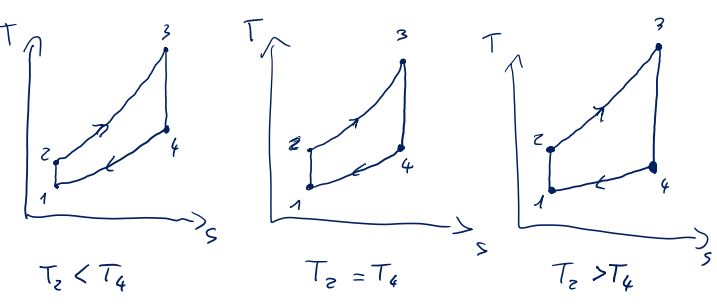
\includegraphics[height=4cm]{../L07/img7.PNG}
\end{center}
L'immagine centrale rappresenta il caso ottimale. Le immagini laterali no, a sinistra l'uscita della turbina è più calda rispetto all'uscita del compressore, a destra l'uscita della turbina è più fredda dell'uscita del compressore.
\subsubsection{Ciclo Joule-Brayton con rigenerazione}
Una delle soluzioni che può portare a un migliroamento del rendimento e del lavoro specifico prodotto che si può applicare al caso $T_2<T_4$, ovvero in cui la temperatura in uscita dalla turbina è maggiore della temperatura in uscita dal compressore.
\begin{center}
    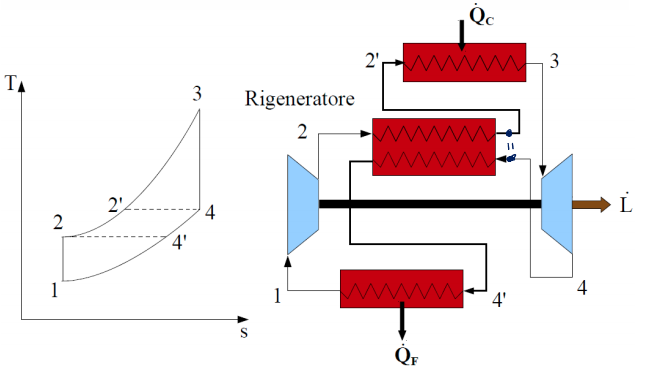
\includegraphics[height=6cm]{../L07/img8.PNG}
\end{center}
La corrente calda in uscita dalla turbina in eccesso viene sfruttata per innalzare la temperatura in uscita dal compressore.\newline
\newline
Per fare questo preriscaldamento durante il riscaldamento (2-3) possiamo utilizzare un rigeneratore (che è uno scambiatore) in modo da trasferire calore fra ciò che esce dalla turbina verso quello che esce dal compressore e quindi recuperare questa energia. Sfruttando questa energia in più il compressore dovrà solo eseguire una trasformazione (2'-3) e non più (2-3) e così si ha un risparmio sulla spesa.\newline
\newline
\subsubsection{Rendimento del ciclo rigenerato ideale}
Per ciclo rigenerato \textbf{ideale} si intende che $T_{2'} = T_4$ (si è recuperata tutta l'energia), che si lavora con gas perfetti e che il ciclo è ideale e simmetrico.
\[
    \eta_{rig} = \frac{\dot{L}}{\dot{Q}_C} = \frac{\dot{L}_T - \dot{L}_C}{\dot{Q}_C} = \frac{(T_3-T_4)-(T_2-T_1)}{(T_3-T_4)} = 1- \frac{T_2-T_1}{T_3-T_4}
\]
\[
    \eta_{rig} = 1- \frac{T_2}{T_3} = 1- \frac{T_2 T_1}{T_3T_1}
\]
\[
    \eta_{rig} = 1- \frac{T_1}{T_3}r_P^{\frac{k-1}{k}}
\]
In una rigenerazione ideale si ha che $T_{2'}=T_4$, mentre in una reale si ha che $T_{2'} < T_4$ (è necessario un salto termico per effettuare lo scambio).
\subsubsection{Ciclo J-B aperto}
\begin{center}
    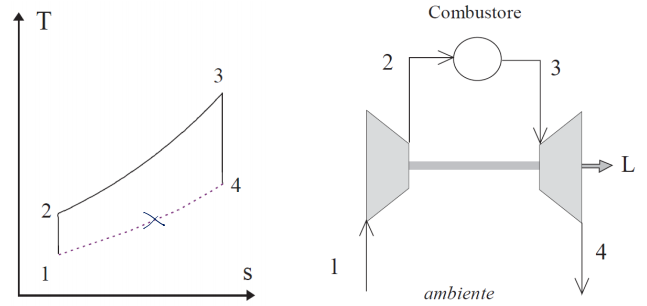
\includegraphics[height=3cm]{../L07/img9.PNG}
\end{center}
\subsection{Ciclo otto}
Il ciclo di Carnot è costituito da due isoentropiche e due isoterme, nel \textbf{ciclo otto}, invece delle isoterme, usiamo due \textbf{isocore} (a pari volume).
\begin{center}
    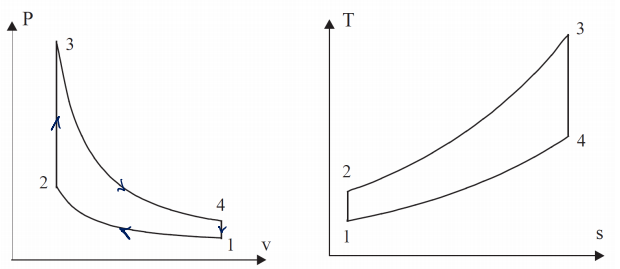
\includegraphics[height=3cm]{../L07/img10.PNG}
\end{center}
(1-2) è la prima isoentropica;\newline
(2-3) seguita dalla prima isocora;\newline
(3-4) seconda isoentropica;\newline
(4-1) seconda isocora.\newline
\newline
Gli scambi di calore avvengono fra (2-3) e (4-1), perchè le isoentropiche sono adiabatiche reversibili e quindi avranno solo scambio di potenza meccanica.\newline
\newline
\subsubsection{Studio termodinamico del ciclo Otto}
Il ciclo otto \textbf{ideale} è costituito da quattro trasformazioni internamente reversibili:
\begin{itemize}
    \item compressione isoentropica;
    \item adduzione di calore a volume costante;
    \item espansione isoentropica;
    \item sottrazione di calore a volume costante.
\end{itemize}
\begin{center}
    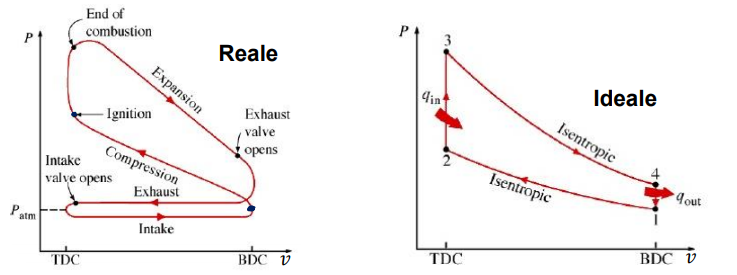
\includegraphics[height=3cm]{../L07/img11.PNG}
\end{center}
A sinistra abbiamo una rappresentazione di un ciclo reale, e a destra quello di un ciclo reale. La differenza principale che c'è fra un ciclo reale e ideale è che in quello ideale non andiamo a considerare il fatto di andare a caricare e scaricare il fluido di lavoro (Exhaust e intake).\newline
\newline
Analiziamo la fase di compressione:
\begin{center}
    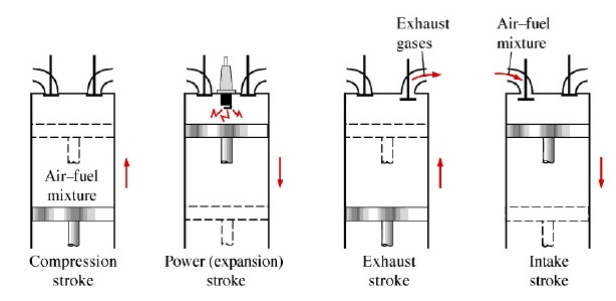
\includegraphics[height=3cm]{../L07/img12.PNG}
\end{center}
\subsubsection{Rendimento termodinamico del ciclo Otto}
Trattiamo il caso di ciclo ideale simmetrico con gas perfetto.\newline
Gli scambi di calore avvengono in un sistema chiuso e in maniera isocora, quindi vale il concetto che
\[
    q_C = u_3- u_2
\]
Ipotizzando costante il calore specifico nell'intervallo di temperatura si ha:
\[
    q_c = c_V(T_3-T_2)
\]
Analogamente l'espressione del calore sottratto vale:
\[
    q_F = u_4-u_1 = c_V(T_4-T_1)
\]
Il rendimento termodinamico del ciclo (ideale) vale:
\[
    \eta_{otto} = \frac{q_c - q_f}{q_c} = 1- \frac{q_f}{q_c} = 1- \frac{T_4-T_1}{T_3-T_2} = 1- \frac{t_1 \left(\frac{T_4}{T_1}-1\right)}{T_2 \left(\frac{T_3}{T_2}-1\right)} = 1- \frac{T_1}{T_2}
\]
Inserendo il bilancio di entropia fra 1 e 2 per i gas perfetti:
\[
    \Delta s_{12} = c_V ln \frac{T_2}{T_1} + R^* ln \frac{V_2}{V_1} = 0
\]
da cui 
\[
    \left(\frac{T_2}{T_1}\right)^{c_V} = \left(\frac{V_1}{V_2}\right)^{R^*}
\]
\[
    \left(\frac{T_2}{T_1}\right) = \left(\frac{V_1}{V_2}\right)^{\frac{R^*}{c_V}} = r_V^{\frac{R^*}{c_V}} = r_V^{k-1}
\]
per cui
\[
    \eta_{otto} = 1- r_V^{1-k}
\]
dove $r_V$ prende il nome di \textbf{rapporto di compressione volumetrico} ($\frac{V_1}{V_2}$, che è $\frac{V_{max}}{V_{min}}$).\newline
\newline
Ci sono spesso problemi nel cercare di migliorare il rendimento del ciclo otto, dovuti al fatto che se si diminuisce troppo $V_min$ (quindi aumentare troppo la pressione massima allo stato 2) , allora si iniziano ad avere combustioni non controllate (spontanee e non volute) della miscela benzina-aria e quindi problemi dal punto di vista del funzionamento (problemi di fattibilità). Nel caso ideale il fluido è aria, e quindi non ci sono problemi, nella pratica è una miscela aria-benzina.
\subsubsection{Lavoro specifico del ciclo otto}
Trattiamo il caso di ciclo ideale simmetrico con gas perfetto.\newline
Con un ragionamento del tutto simile al precedente:
\[
    l = c_V(T_3-T_4) -c_V(T_2-T_1)
\]
\[
    l = c_VT_3\left(1-\frac{T_4}{T_3}\right) - c_V T_1 \left(\frac{T_2}{T_1}-1 \right)
\]
\[
    l = c_V T_3 \left(1- \frac{1}{r_V^{k-1}}\right) - c_V T_1 (r_V^{k-1} - 1)
\]
Il lavoro è ottimale quando il rapporto di compressione vale
\[
    r_{V,opt} = \left(\frac{T_3}{T_1}\right)^{\frac{1}{2(k-1)}}
\]
\subsection{Ciclo Diesel}
Il \textbf{ciclo diesel} è simile al ciclo otto, ed è composto da \textbf{due isoentropiche}, \textbf{una isocora} e \textbf{una isobara}
\begin{center}
    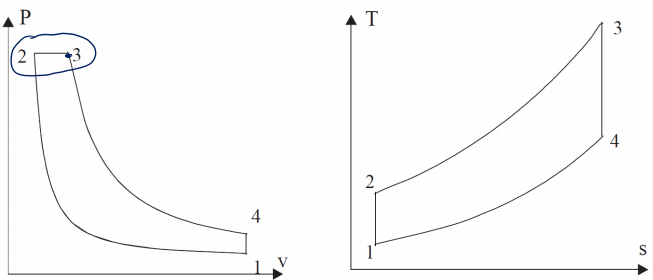
\includegraphics[height=4cm]{../L07/img13.PNG}
\end{center}
\subsubsection{Rendimento termodinamico del ciclo Diesel}
Consideriamo anche in questo caso un ciclo \textbf{ideale} simmetrico di un gas perfetto.
\[
    \eta_{Diesel} = \frac{L}{Q_C} = 1- \frac{Q_F}{Q_C} = 1- \frac{c_V(T_4-T_1)}{c_P(T_3-T_2)} = 1- \frac{c_V T_1\left(\frac{T_4}{T_1}-1\right)}{c_P T_2 \left(\frac{T_3}{T_2}-1\right)}
\]
La cosa fondamentale che cambia rispetto al ciclo otto è che $Q_F$ è lo scambio termico lungo una isocora.\newline
Definiamo:
\[
    r = \frac{V_1}{V_2} \;\;\;\text{che è uguale a dire }\; \frac{V_max}{V_min}
\]
\[
    z = \frac{V_3}{V_2} \;\;\;\text{che è uguale a dire}\; \frac{V_{fine \; combustione}}{V_{inizio \; combustione}}
\]
dove $r$ è il \textbf{rapporto di comrpessione volumetrico} e $z$ è il \textbf{rapporto di combustione}.\newline
Allora possiamo dire:
\[
    \eta_{Diesel} = 1- \frac{1}{r^{k-1}} \frac{1}{k} \frac{(z^k -1)}{(z-1)}
\]
Confrontando il rendimento del ciclo Diesel con quello del ciclo Otto a parità di compressione volumetrica, ci si accorge che il ciclo Otto ha un rendimento maggiore.
\subsubsection{Vantaggi del motore Otto rispetto al motore Diesel}
\begin{itemize}
    \item Maggiore leggerezza;
    \item Maggiore frequenza di rotazione;
    \item Minore rumorosità;
    \item Minore rendimento globale;
    \item Brusco calo di rendimento al diminuire del carico;
    \item Utilizzo di combustibili più pregiati
\end{itemize}
\subsection{Ciclo Joule-Brayton inverso}
Il \textbf{ciclo Joule-Brayton inveso} è un ciclo \textbf{frigorifero} (per macchine operatrici) simmetrico costituito da \textbf{due isoentropiche} e \textbf{due isobare}.
\begin{center}
    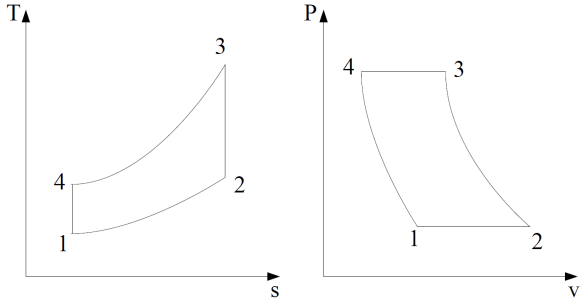
\includegraphics[height=4cm]{../L07/img14.PNG}
\end{center}
\subsubsection{Efficienza del ciclo}
\[
    \epsilon = \frac{\dot{Q}_F}{\dot{Q}_C -\dot{Q}_F}
\]
\[
    \epsilon = \left(\frac{T_2-T_1}{(T_3-T_4) - (T_2-T_1)}\right)
\]
\[
    \epsilon = \frac{T_2}{T_3-T_2} = \frac{T_1}{T_4-T_1} = \left(  \frac{1}{r_P^{\frac{k-1}{k}}-1}  \right)
\]
\textbf{solo per cicli simmetrici}:
\begin{itemize}
    \item alta efficienza quando $r_P \rightarrow 1$ però aumentano le dimensioni dell'impianto;
    \item miglioramento ottenibile con l'impiego della rigenerazione;
\end{itemize}
\subsection{Ciclo Stirling}
\textbf{Ciclo simmetrico costituito da due isoterme e due isocore}
\subsection{Ciclo Ericsson}
\textbf{Ciclo simmetrico costituito da due isoterme e due isobare}
\subsection{Riassunto dei cicli}
\begin{center}
    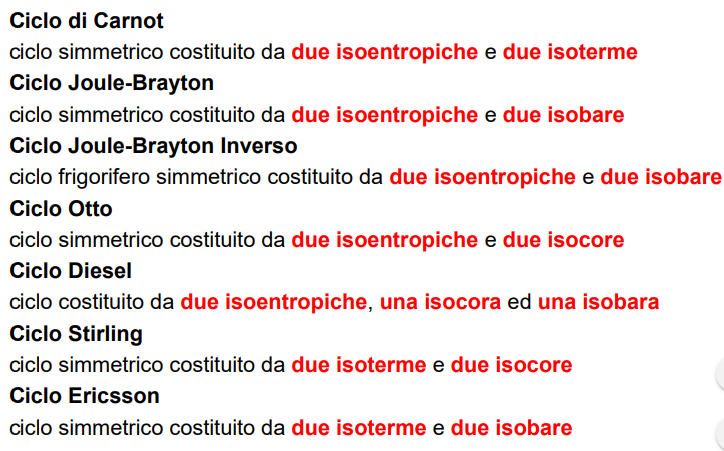
\includegraphics[height=6cm]{../L07/img15.PNG}
\end{center}

    \newpage
    \url{../pdf/Lezioni/L08-Cicli a vapore-con-annotazioni.pdf}
    \section{L08-Cicli a vapore}
\subsection{Cicli termodinamici a vapore}
Nei cicli a vapore il fluido di lavoro subisce trasformazioni di fase.
\subsubsection{Ciclo di Carnot a vapore}
Il ciclo di Carnot è il ciclo ideale che permette di avere rendimento massimo della macchina ciclica con i serbatoi di calore che si ha a disposizione.\newline
\newline
E' composto da due isoentropiche e due isoterme (un quadrato nel diagramma temperatura e entropia).\newline
\newline
Abbiamo visto che ci sono molti svantaggi nell'impiegare il ciclo di Carnot nella versione monofase (cioè a gas): per prima cosa la trasformazione isoterma (superfici grandi e trasformazioni lente) ha caratteristiche opposte a quelle isoentropiche (superfici ridotte e trasformazioni veloci), inoltre il lavoro specifico (l'area sottesa nel diagramma pressione-volume) è molto basso.\newline
\newline
Invece, inseriamo il ciclo di Carnot all'interno di una zona bifase di una sostanza facendo corrispondere gli stati $2$ e $3$ a stati di liquido saturo e vapore saturo rispettivamente, otteniamo due isoentropiche ($1-2$ e $3-4$) e due isoterme ($2-3$ e $4-1$):
\begin{center}
    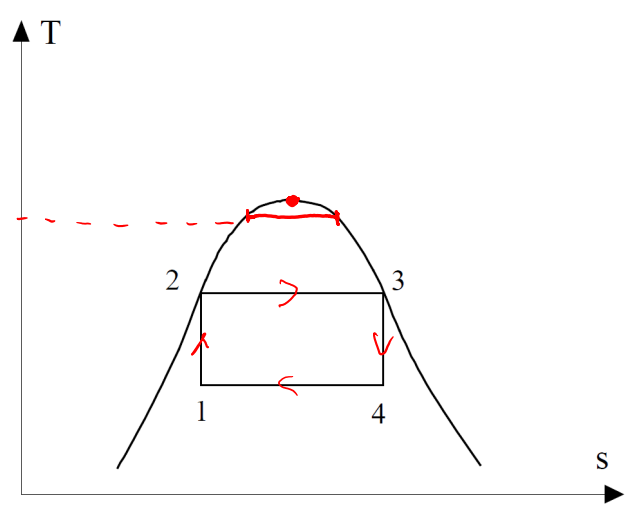
\includegraphics[height=4cm]{../L08/img1.PNG}
\end{center}
\textbf{Vantaggi}: 
\begin{itemize}
    \item Ricordiamo che se in zona bifase abbiamo temperatura costante (nelle isoterme) allora anche la pressione è costante. Ciò comporta che le isoterme siano anche isobare e dal punto di vista pratico le isobare sono facili da realizzare nella realtà.
    \item Un altro vantaggio di usare il ciclo di Carnot nella zona bifase è che c'è un notevole incremento di variazione di entalpia (dovuta all'entalpia di transizione), per cui se si guardasse l'area sottesa nel siagramma pressione-volume vedremmo che il lavoro specifico è alto.
\end{itemize}
\textbf{Svantaggi}:
\begin{itemize}
    \item E' molto dispendioso e difficile da realizzare la compressioen $1-2$.
    \item L'espansione $3-4$ è conveniente se il titolo $x_4 > 0,9$.
\end{itemize}
\subsubsection{Caratteristiche di un fluido di lavoro per il ciclo a vapore}
Per ridurre, a parità di potenza, la portata di fluido e quindi le dimensioni (e il costo) dell'impianto:
\begin{itemize}
    \item Elevata \textbf{massa volumica};
    \item Elevata \textbf{entalpia di transione di fase};
\end{itemize}
Al punto critico l'entalia di evaporazione è nulla:
\begin{itemize}
    \item Elevata \textbf{temperatura critica};
\end{itemize}
Evitare la presenza di una fase solida:
\begin{itemize}
    \item Temperature del \textbf{punto triplo} inferiore alla temperatura minima del ciclo;
\end{itemize}
Ridurre costi materiali e allungare ciclo di vita dell'impianto:
\begin{itemize}
    \item Fluido \textbf{non corrosivo};
\end{itemize}
Ridurre rischi ambientali:
\begin{itemize}
    \item Fluido \textbf{non tossico};
\end{itemize}
Aumentare sicurezza dell'impianto:
\begin{itemize}
    \item Fluido \textbf{chimicamente stabile};
\end{itemize}
Ridurre i costi:
\begin{itemize}
    \item Facilmente \textbf{reperibile e di basso costo};
\end{itemize}
Vapore in uscita dalla turbina con elevato titolo:
\begin{itemize}
    \item \textbf{Elevata pendenza} nel piano $T-s$ della curva limite superiore (più la curva è pendente e più il titolo allo stato $4$ sarà elevato);
\end{itemize}
Evitare infiltrazioni di gas incondensabili e conseguente necessità di apparecchiature atte al mantenimento dell'opportuno grado di vuoto (la temperatura al condensatore deve essere vicina a quella del serbatoio di calore inferiore per avere una limitazione delle irreversibilità):
\begin{itemize}
    \item \textbf{Pressione di condensazione} superiore alla pressione atmosferica;
\end{itemize}
\ \newline
\textbf{Nessun fluido} possiede tutte le proprietà citate. il fluido più adatto dipende dalle condizioni di contorno, in particolare delle temperatura delle sorgenti.\newline
\newline
\textbf{Cicli motore}: Tipicamente viene usata l'acqua che possiede le principali proprietà.\newline
\newline
\textbf{Cicli inversi (frigoriferi)}: Ci sono molti fluidi fra cui scogliere, per esempio:
\begin{itemize}
    \item Ammoniaca $NH_3$ (ma è tossico);
    \item Clorofluorocarburi (CFN o freon) (ma sono dannosi per l'ozono) (esempi: R11, R12);
    \item Clorofluoroidrocarburi (HCFC) e Fluoroidrocarburi (HFC) (sono meno dannosi per l'ozono) (esempi: R22, R123, \textbf{R134a})
\end{itemize}
\ \newline
Vediamo una tabella che mostra le caratteristiche di acqua e R134a, i due fluidi che useremo in questo corso:
\begin{center}
    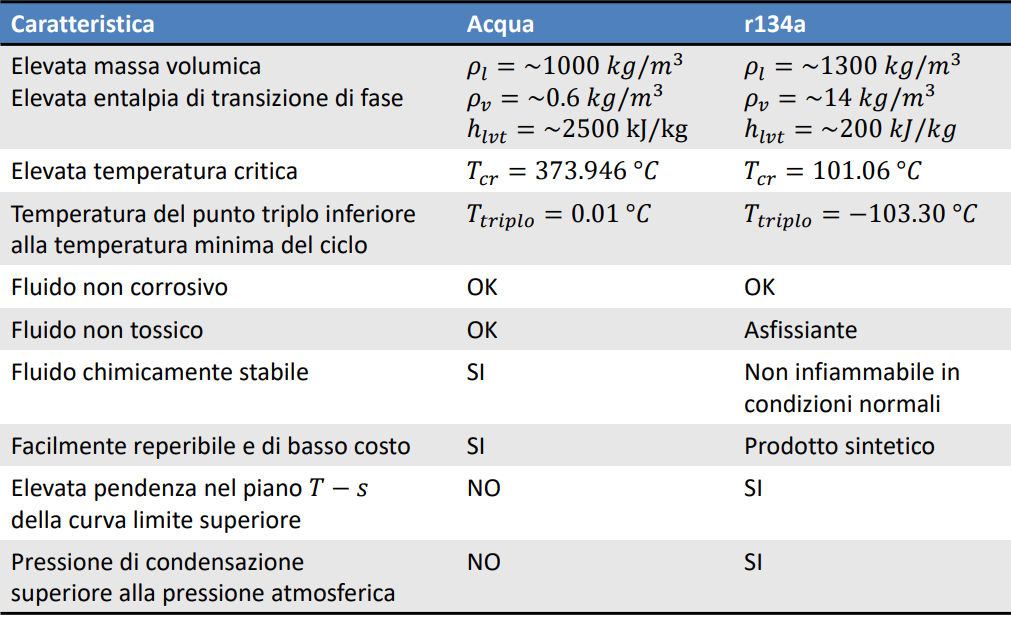
\includegraphics[height=6cm]{../L08/img2.PNG}
\end{center}
Vediamo ora i diagrammi $T-s$ (che possono anche essere usati al posto delle tabelle... le tabelle sono più precise):
\begin{center}
    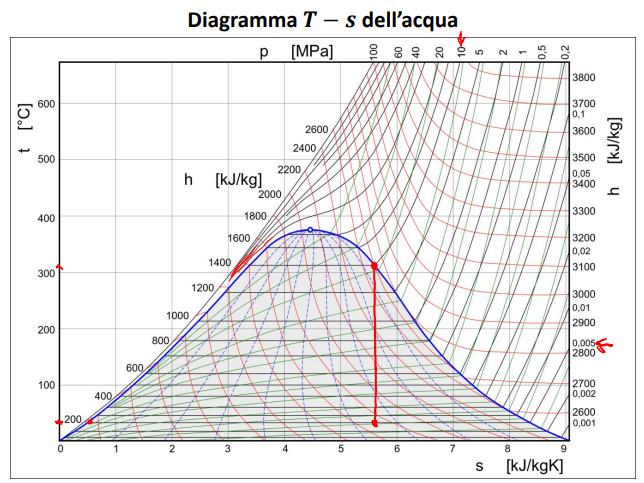
\includegraphics[height=5cm]{../L08/img3.PNG}
\end{center}
In azzurro: curva di saturazione, notiamo che la parte a destra di questa curva non è particolarmente ripida;\newline
Le curve nere sono le isobare, in cui si leggono le pressioni in mega pascal alcune in alto e alcune a destra;\newline
Tutte le righe orizzontali sono isoterme, e quelle verticali sono isoentropiche.\newline
Le curve rosse sono isoentalpiche (a parità di entalpia); \newline
Le curve verdi sono isovolumiche;\newline
Le curve azzurre tratteggiate sono quelle di isotitolo.
\begin{center}
    \includegraphics[height=5cm]{../L08/img4.PNG}
\end{center}
La curva nera marcata è la curva di saturazione: per l'r124a abbiamo una forte pendenza nella parte destra della curva di saturazione, questo vuol dire che si ha in uscita un alto titolo;\newline
Le curve verdi sono isovolumiche;\newline
Quelle in rosso sono isobare;\newline
Quelle azzurre sono le isoentalpie;\newline
quelle nere sono isotitolo;
\subsection{Ciclo Rankine}
\subsubsection{Ciclo Rankine semplice (a vapore saturo)}
Il ciclo Rankine semplice rappresenta un metodo per rendere realizzabile il ciclo di Carnot. La compressione $1-2$ nel ciclo di Carnot, all'interno del bifase, è un'operazione molto dispendiosa con molte irreversibilità interne. Per ovviare a questo porblema, viene fatta proseguire la condensazione fino allo stato $1$ della seguente immagine:
\begin{center}
    \includegraphics[height=4cm]{../L08/img5.PNG}
\end{center}
arrivati allo stato $1$ si ha un monofase liquido. Per far salire la pressione di questo liquido si usa ora una \textbf{pompa} fino a raggiugnere uno stato $2$.\newline
Nota: la rappresentazione della compressione $1-2$ non è fedele in quanto le isobare, nella zona dello stato liquido, sono molto vicine alla curva di saturazione (confrontare con il diagramma $T-s$ visto precedentemente). Per visualizzare meglio il ciclo spostiamo lo stato $2$ in modo che sia ben chiaro.
\begin{center}
    \includegraphics[height=5cm]{../L08/img6.PNG}
\end{center}
Arrivati allo stato $2$ si esegue una trasformazione isobara e si raggiunge lo stato $3$. le trasformazione $2-3$ e $3-4$ rappresentano lo scambiatore di calore, ma nel disegno dello schema di impianto, questo scambiatore di lavoro viene rappresentato come due cerchi collegati da una serie di connessioni. Questo componente è un generatore di vapore ed è posto in verticale perchè nel contenitore inferiore c'è acqua liquida, attraversando i vari tubi diventa vapore e giunge nel contenitore superiore. Per la gravità se ci fosse ancora acqua in stato liquido nel contenitore superiore, questa cadrebbe in modo da tornare a quello inferiore e ripetere il processo.\newline
\newline
Nell'espansione $4-5$ rimane il problema che il titolo in $5$ può essere minore di $0,9$ e quindi causare problemi (vedi svantaggi del ciclo di Carnot a vapore).\newline
\newline
Il lavoro totale uscente è il lavoro prodotto dalla turbina meno il lavoro che si spende nella pompa.
\subsubsection{Ciclo Rankine}
Il ciclo Rankine completo presenta una modifica ulteriore: per evitare di avere problemi di titolo minore di $0,9$ allo stato $5$ (all'uscita della turbina) ed aumentare il rendimento, si effettua il surriscaldamento del vapore $(4-5)$:
\begin{center}
    \includegraphics[height=4cm]{../L08/img7.PNG}
\end{center}
Notiamo che da $2$ a $5$ si è sulla stessa isobara: la pressione su $2,3,4,5$ è la stessa.\newline
\newline
L'espansione della turbina avviene quindi in $5-6$ e lo stato $6$ (cioè l'uscita della turbina) avrà un titolo maggiore rispetto al caso di ciclo Rankine semplice.\newline
\newline
Questo riscaldamento aggiuntivo aumenta la potenza erogata dalla turbina (si ha un salto entalpico maggiore fra $5-6$), ma dall'altro lato si avrà una spesa maggiore, ma comunque si avrà un rendimento più alto
\[
    \eta = 1- \frac{\dot{Q}_F}{\dot{Q}_C} = 1- \frac{h_6-h_1}{h_5-h_2}
\]
\ \newline
Dal punto di vista impiantistico la differenza è che il flusso in uscita dal generatore di vapore viene deviato verso il generatore di vapore in modo da rimetterlo a contatto con una fonte di calore.
\begin{center}
    \includegraphics[height=5cm]{../L08/img8.PNG}
\end{center}
\ \newline
\textbf{Soluzioni per migliorare il rendimento del ciclo Rankine}\newline
\begin{itemize}
    \item \textbf{Riduzione della pressione di condensazione}:\newline
    Cioè si cerca di portare la temperatura nel condensatore a quella dell'ambiente (cioè la sorgente di calore inferiore), ovvero stiamo cercando di abbassare la trasformazione $6-1$.
    \begin{center}
        \includegraphics[height=3cm]{../L08/img9.PNG}
    \end{center}
    Nel condensatore se si abbassa la temperatura di saturazione si abbassa anche la pressione.\newline
    \newline
    Il limite principale di questo miglioramente sono i limiti tecnologici: limiti tecnologici per le infiltrazioni quando $P < P_{atm}$ (tipico quando si utilizza acqua)..\newline
    \newline
    Siccome si ha una differenza di temperatura maggiore nella trasformazione della turbina, allora si ha un aumento del lavoro prodotto, contemporaneamente si avrà anche un innalzamento del consumo della pompa, ma la turbina produce di più di quanto la pompa consumi.\newline
    \newline
    Avremo tendenzialmente un rendimento del ciclo maggiore, ma anche un rendimento della macchina termica migliore (si diminuiscono le irreversibilità esterne).
    \item \textbf{Aumento della temperatura finale di surriscaldamento}:\newline
    \begin{center}
        \includegraphics[height=3cm]{../L08/img10.PNG}
    \end{center}
    Si aumenta la temperatura massima del ciclo, in modo che aumenti il salto entalpico della turbina e quindi aumenti il lavoro prodotto. Il lavoro prodotto dalla turbina è maggiore della quantità di calore necessaria da fornire e quindi si ha un miglioramento del rendimento.\newline
    \newline
    Inoltre si ha pure un aumento del titolo d'uscita dalla turbina. \newline
    \newline
    I limiti dell'aumento della temperatura sono di tipo tecnologico ($T_{max} = 650^o C$).
    \item \textbf{ Aumento della pressione di vaporizzazione}:
    \begin{center}
        \includegraphics[height=3cm]{../L08/img11.PNG}
    \end{center}
    Questa soluzione consente di ridurre la potenza termita scambiata a parità di produzione di energia meccanica della turbina.\newline
    \newline
    Per aumento della pressione di vaporizzazione si intende un aumento della temperatura in $3$ e in $4$.\newline
    \newline
    Il lavoro prodotto rimane simile, ma si riduce il calore fornito $\dot{Q}_C$ per passare da $2$ a $5$ (il salto entalpico è minore) e di conseguenza si aumenta il rendimento.\newline
    \newline
    Un aspetto negativo è che si riduce il titolo in uscita dalla turbina.\newline
    \newline
    I limiti di questa soluzione sono legati ai costi (maggiore costo di impianto per restistere a pressioni più elevate) e al punto critico, per cui la pressione massima accettabile è $P_{max} = 200 bar$.
    \item \textbf{Surriscaldamenti ripetuti}:
    \begin{center}
        \includegraphics[height=3cm]{../L08/img12.PNG}
    \end{center}
    Nel ciclo Rankine ne abbiamo solo uno di surriscaldamento, ma se ne possono fare di più. Nell'immagine è rappresentato un ciclo Rankine con due riscaldamenti, chiamato anche Rankine con risurriscaldamento.\newline
    \newline
    $4-5$ è l'isobara ad alta pressione e $4'-5'$ è l'isobara a bassa pressione.\newline
    \newline
    Aumenta il lavoro prodotto; aumenta il calore fornito $\dot{Q}_C$; aumenta il rendimento; aumenta il titolo in uscita dalla turbina; necessità di una turbina a più stadi (diverse sezioni nella turbina, una per ogni trasformazione a pressione diversa).
    \begin{center}
        \includegraphics[height=4cm]{../L08/img13.PNG}
    \end{center}
    Vediamo nell'immagine la turbina HP (high pressure) e poi la tubrina LP (low pressure).
    \item \textbf{Rigenerazione}:\newline
\end{itemize}
\subsection{Ciclo frigorifero a vapore}
\subsubsection{Ciclo di Carnot inverso a vapore}
\begin{center}
    \includegraphics[height=4cm]{../L08/img14.PNG}
\end{center}
$1-2$ è un espansione non problematica, $3-4$ è una compressione (di un vapore con un po' di liquido, cioè un bifase) che può condurre ad un elevata erosione del compressore per via di alte irreversibilità, $2-3$ è l'evaporazione, e $4-1$ è la condensazione.
\subsubsection{Ciclo frigorifero a vapore teorico}
\begin{center}
    \includegraphics[height=4cm]{../L08/img15.PNG}
\end{center}
$3-4$ è una compresisone di un vapore saturo/surriscaldato preferibilmente. Questa compressione ha comunque irreversibiltà ma molto minori rispetto al caso bifase del ciclo di Carnot.\newline
\newline
L'espansione $1-2$ avviene con una turbina, e non è conveniente nel mondo reale perche è difficile da usare, perchè il fluido è inizialmente in fase liquida e deve evaporare. Questa evaporazione fa danni strutturali ai componenti.
\subsubsection{Ciclo frigorifero a vapore} 
\begin{center}
    \includegraphics[height=4cm]{../L08/img16.PNG}
\end{center}
L'espansione $1-2$ è isoentalpica, non viene scambiato calore, non c'è generazione di entalpia, ma c'è produzione di entropia. (è tratteggiata perchè è irreversibile).
\begin{center}
    \includegraphics[height=5cm]{../L08/img17.PNG}
\end{center}
L'evaporatore e il condensatore sono rappresentati come scambiatori di calore (per ricordarsi quale è quale, tenere presente che il condensatore rilascia calore, mentre l'evaporatore ne assorbe).\newline
Notiamo che l'evaporatore ha posizione opposta rispetto a quella del ciclo Rankine.\newline
    \newpage
    \url{../pdf/Lezioni/L09-Trasmissione del calore.pdf}
    \section{L09-Trasmissione del calore}
    \newpage
    \part{NOTE SUGLI ESERCIZI}
    \newpage
    \url{../pdf/Materiale extra/2004_Inzoli,Colombo_Fisica Tecnica - Eserciziario.pdf}
    \section{Linee guida per gli esercizi}
\subsection{Impostazione del problem}
\begin{itemize}
    \item Leggere bene il testo del problema.
    \item Effettuare una schematizzazione del problema: identificare il tipo di sistema, il suo
    contorno, la sostanza evolvente nel sistema, gli scambi di massa, calore e lavoro con
    l’ambiente e la loro direzione.
    \item Scrivere i dati forniti dal testo del problema, e le incognite da ricavare per risolverlo.
    Convertire i dati in unità di misura congruenti e conformi al Sistema Internazionale.
    \item Se avvengono trasformazioni termodinamiche, rappresentarle qualitativamente su un
    diagramma opportuno.    
\end{itemize}
\subsection{Soluzione del problema}
\begin{itemize}
    \item Scrivere i bilanci di massa, energia ed entropia per il volume di controllo considerato.
    Elencare le ipotesi applicabili al sistema (riguardo la natura del contorno del sistema, delle
    trasformazioni che avvengono al suo interno, delle sostanze delle quali è composto), e
    semplificare i bilanci di conseguenza, ponendo attenzione alle convenzioni di segno.
    \item Scrivere la soluzione analitica del problema.
    \item Risolvere il problema numericamente. Si raccomanda di scrivere sempre le unità di misura
    delle grandezze calcolate e di fare l’analisi dimensionale delle equazioni scritte.
    \item Fare sempre caso alla ragionevolezza dei risultati  
\end{itemize}
\subsection{Unità di misura}
\begin{center}
    \includegraphics[height=5cm]{../L01/img10.PNG}
\end{center}
\begin{center}
    \includegraphics[height=7cm]{../L01/img11.PNG}
\end{center}
\begin{center}
    \includegraphics[height=5cm]{../L01/img12.PNG}
\end{center}
\begin{center}
    \includegraphics[height=5cm]{../L01/img13.PNG}
\end{center}
\section{Equazioni di bilancio per i sistemi chiusi}
Un \textbf{sistema chiuso} è un sistema per il quale non sono consentiti scambi di massa attraverso il suo contorno. Per tale sistema non è in uso applicare \textbf{equazioni di bilancio di massa} essendo implicita la sua conservazione nella definizione di sistema chiuso.\newline
\newline
Nelle soluzioni di problemi con sistemi chiusi le equazioni fondamentali sono \textbf{l'equazione di bilancio energetico} e \textbf{l'equazione di bilancio entropico} che assumono la forma:
\[
    \Delta U = Q^\leftarrow  -L^\rightarrow  
\]
\[
    \Delta S = S_Q + S_{irr}
\]
cioè la variazione di energia interna è pari alla differenza tra il calore entrante nel sistema e il lavoro ceduto dal sistema; la variazione di entropia è pari alla somma della entropia $S_Q$ entrante attraverso il contorno del sistema con il calore Q e della quantità $S_{irr}$ generata all'interno del sistema per irreversibilità. Questa ultima quantità è sempre positiva e tende a zero col tendere dei processi alla reversibilità. Inoltre il segno del termine $S_Q$ è sempre uguale al segno di $Q$.\newline
\newline
L'\textbf{energia interna} e l'\textbf{entropia} sono proprietà \textbf{estensive e additive}. Quindi dato un sistema $Z$ composto da due sottosistemi $A$ e $B$, posso scrivere:
\[
    \Delta U_Z = \Delta U_A + \Delta U_B = Q_Z^\leftarrow  - L_Z^\rightarrow  \;\;\;\;\;\;\;\;\;\;\Delta S_Z = \Delta S_A + \Delta S_B = S_{Q,Z} + S_{irr,Z}
\]
\ \newline
\newline
Se il \textbf{lavoro scambiato} è lavoro meccanico quasi-statico (internamente reversibile), è determinabile con l'espressione:
\[
    L = \int_{i}^{f} P dV
\]
Questa espressione è integrabile se è nota l'equazione della trasformazione ovvero la funzione:
\[
    P = P(V)
\]
\ \newline
Il \textbf{calore scambiato}, nell'ipotesi di trasformazione quasi-statica, può essere determinato avendo noto il calore specifico della trasformazione:
\[
    Q = M c_x (T_2-T_1)
\]
\ \newline
L'\textbf{energia interna} di un sistema in uno stato di equilibrio può essere espressa in funzione di altre proprietà intensive ed estensive specifiche del sistema come la temperatura, il volume specifico, la pressione. Particolarmente utili sono i due seguenti casi in cui è possibile esprimere in una forma analitica elementare il legame funzionale tra la variazione di energia interna tra due stati di equilibrio e la variazione di temperatura. \newline
\textbf{Gas perfetto}: $\Delta u = c_V (T_2 - T_1)$\newline
\textbf{Liquido incomprimibile perfetto}: $\Delta u = c(T_2-T_1)$\newline
Inoltre:
\begin{itemize}
    \item Per un sistema isolato $\Delta U_{isolato} = 0$.
    \item Per un sistema che subisce una trasformazione ciclica: $\Delta U_{ciclo} = 0$
\end{itemize}
\ \newline
\newline
Il caso di trasformazioni quasi-statiche a pressione costante o trasformazioni irreversibili in un sistema con stato iniziale e finale alla stessa pressione consente di scrivere l’equazione di bilancio energetico per il sistema chiuso come:
\[
    \Delta H = Q \;\;\;\;\;\;\;\;\;\;\;\;\;\;\;\text{dove $h = u + Pv$}\;
\]
Per esempio la miscelazione adiabatica e isobara di due sottosistemi produce uno stato finale caratterizzato da un valore di entalpia totale pari alla somma delle entalpia iniziale dei due sottosistemi. \newline
L'\textbf{entalpia specifica} di un sistema in uno stato di equilibrio può essere espressa
in funzione di altre proprietà intensive ed estensive specifiche del sistema come la
temperatura, il volume specifico, la pressione. Particolarmente utili sono i due seguenti casi
in cui è possibile esprimere in una forma analitica elementare il legame funzionale tra la
variazione di entalpia specifica tra due stati di equilibrio e la variazione di temperatura. \newline
\textbf{Gas perfetto}: $\Delta h = c_P (T_2 - T_1)$\newline
\textbf{Liquido incomprimibile perfetto}: $\Delta h = c(T_2-T_1) + v(P_2-P_1)$\newline
\newline
L'\textbf{entropia} è una proprietà del sistema e quindi dipende solo dallo stato del sistema: ne consegue che noti gli stati iniziale e finale di un processo, la determinazione della variazione di entropia prescinde dalla conoscenza di qualsiasi dettaglio del processo (ivi compresa la sua reversibilità). Particolarmente utili sono i due seguenti casi in cui è possibile esprimere in una forma analitica elementare il legame funzionale tra l'entropia e altre proprietà del sistema. Per il gas perfetto sono possibili 3 diverse espressioni che fanno uso di 3 diverse coppie di coordinate termodinamiche indipendenti. \newline
\textbf{Gas perfetto}:
\[
    \begin{matrix}
        \Delta s = c_P ln \frac{T_2}{T_1} - R^* ln \frac{P_2}{P_1} \;\;\;\;\;\;\;\;\;\;\;\;\;\;\;\Delta s = c_V ln \frac{T_2}{T_1} + R^* ln \frac{V_2}{V_1}\\
        \Delta s = c_V ln \frac{P_2}{P_1} + c_P ln \frac{V_2}{V_1}
    \end{matrix}
\]
\textbf{Liquido incomprimibile perfetto}: $\Delta s = c ln \frac{T_2}{T_1}$\newline
Inoltre:
\begin{itemize}
    \item Per definizione la variazione di entropia di un serbatoio di lavoro ($\Delta S_{SL}$) è nulla.
    \item Per definizione la variazione di entropia di un serbatoio di calore ($\Delta S_{SC}$) ha solo la componente reversibile, gli scambi avvengono con trasformazioni quasi-statiche (internamente reversibili).
    \item Un processo è impossibile da realizzare nel momento in cui $S_{irr} < 0$.
    \item La variazione di entrpia per una trasformazione reversibile è data da $\Delta S = \int_{i}^f \frac{1}{T} \delta Q_{rev}^\leftarrow$ (per i casi in cui $T$ è costante, allora $\Delta S = \frac{Q}{T}$).
    \item La variazione di entropia totale di un sistema isolato sede di trasformazioni termodinamiche è
    sempre maggiore di zero e tende a zero con il tendere dei processi alla reversibilità $\Delta S_{isolato} \geq 0$.
    \item $S_{irr} \geq 0$ è sempre maggiore di zero e il segno di $S_{Q}^\leftarrow $ è uguale al segno di $Q^\leftarrow$
\end{itemize}
\ \newline
\newline
\textbf{L’energia interna, l’entalpia e l’entropia} sono proprietà del sistema e quindi dipendono solo
dallo stato del sistema: ne consegue che noti gli stati iniziale e finale di un processo, la
determinazione della loro variazione prescinde dalla conoscenza di qualsiasi dettaglio del
processo (ivi compresa la sua reversibilità). Non è invece possibile determinare \textbf{il lavoro ed il
calore} scambiato dal sistema nel caso in cui si conoscano solo stato iniziale e finale e in tal caso non si ricorre pertanto alla scrittura del bilancio di energia (primo principio) e di entropia (secondo principio) che risulterebbero
indeterminati, ma si ricorre alle equazioni di stato (per i gas perfetti o per i liquidi incomprimibili perfetti\dots) che utilizzano solamente dati dello stato iniziale e finale.
\section{Stati monofase: equazioni di stato e trasformazioni}
Le sostanze nello stato monofase possono schematicamente essere suddivise in sostanze nello
stato aeriforme, liquido o solido. I modelli di equazioni di stato sono, in prima
approssimazione, ricondotti a modelli ideali o modelli reali.
\subsection{Gas ideali}
Le equazioni di stato dei \textbf{gas ideali} sono:
\[
    PV=MR^*T
\]
\[
    U=U(T) \;\;\;\;\;\;\;\;\;\;\;\;\Delta U = M c_V \Delta T \rightarrow \Delta u = c_V \Delta T
\]
La costante $R^*$ rappresenta la costante del gas ed è determinabile con la relazione:
\[
    R^* = \frac{R}{M_m}
\]
\[
    R=8314 [J/kmole K] =\text{costatne universale dei gas}\; \;\;\;\;\;\;\;\;\;\;M_m = \text{massa molare}\;
\]
\begin{center}
    \includegraphics[height=3cm]{../NOTE SUGLI ESERCIZI/img1.PNG}
\end{center}
La grandezza $c_V$ rappresenta il calore specifico a volume costante funzione del gas e della sua
struttura molecolare. Qualora il calore specifico a volume costante possa assumersi indipendente dalla temperatura (e quindi costante) si parla di gas perfetto.
\subsection{Liquidi e solidi incomprimibili ideali}
Le equazioni di stato dei fluidi incomprimibili ideali (liquidi e solidi) sono:
\[
    v = costante
\]
\[
    U=U(T)  \;\;\;\;\;\;\;\;\;\;\;\;\Delta U = M c \Delta T \rightarrow \Delta u = c \Delta T
\]
dove $c$ è il calore specifico della sostanza.
\subsection{Gas reali}
Una possibile equazione di stato dei gas reali è:
\[
    Pv = ZRT
\]
dove $Z$ è il fattore di compressibilità. Tale coefficiente è determinabile attraverso il diagramma generalizzato che riposta il fattore di compressibilità in funzione della pressione e della temperatura ridotta. La pressione e la temperatura ridotte sono valori adimensionali ottenuti dalle relazioni:
\[
    P_R = \frac{P}{P_{cr}} \;\;\;\;\;\;\;\;\;\;\;\;\;\;\;T_R = \frac{T}{T_{cr}}
\]
in cui $P_{cr}$ e $T_{cr}$ rappresentano i valori di pressione e temperatura nello stato critico.
\begin{center}
    \includegraphics[height=5cm]{../NOTE SUGLI ESERCIZI/img2.PNG}
\end{center}
\subsection{Liquidi e solidi reali}
Le equazioni di stato dei liquidi e solidi reali sono formulate in forma differenziale:
\[
    dv = \beta v \cdot dT - K_Tv \cdot  dP
\]
\[
    \text{Coefficiente di dilatazione termica isobaro}\;\;\;\beta = \frac{1}{v} \left(\frac{\delta v}{\delta T}\right)_P
\]
\[
    \text{Coefficiente di comprimibilità isotermo}\;\;\;K_T = - \frac{1}{v} \left(\frac{\delta v}{\delta P}\right)_T
\]
Siccome $\beta$ e $K_T$ possono essere considerati costanti per ampi intervalli di temperatura e di pressione, la precedente relazione differenziale è integrabile e lo stato calcolabile.
\begin{center}
    \includegraphics[height=3cm]{../NOTE SUGLI ESERCIZI/img3.PNG}
\end{center}
\subsection{Trasformazioni politropiche}
Le \textbf{trasformazioni politropiche} sono trasformazioni termodinamiche \textbf{internamente reversibili}
proprie dei \textbf{gas perfetti} e caratterizzate dall’avere un calore specifico $c_x$ \textbf{costante}.\newline
\newline
L’equazione della politropica in coordinate P,v risulta
\[
    Pv^n = costante \;\;\;\;\;\;\;\;\;\;\text{dove \textbf{l'indice della politropica} è}\;\;\;n = \frac{c_x - c_P}{c_x - c_V}
\]
Con l’ausilio dell’equazione di stato dei gas ideali è possibile ottenere espressioni
dell’equazione della politropica in coordinate T,P e T,v: 
\[
    P^{1-n}T^n = costante
\]
\[
    Tv^{n-1} = costante
\]
Si distinguono alcune trasformazioni elementari particolarmente utili tra le politropiche: 
\begin{center}
    \begin{tabular}{ |c|c|c|c| } 
        \hline
        Trasformazione & $c_x$ & $n = \frac{c_x - x_P}{c_x - c_V}$ \\
        \hline
        Isoterma ($T = costante$) & $\pm \infty$ & $1$ \\ 
        Isocora ($v = costante$) & $c_V$ & $\pm \infty$\\ 
        Isobara ($P = costante$) & $c_P$ & $0$\\ 
        Adiabatica ($q = costante$) & $0$ & $k= \frac{c_P}{c_V}$\\ 
        \hline
    \end{tabular}
\end{center}
\ \newline
Si ricorda che il \textbf{primo principio} è \textbf{sempre applicabile} ed essendo la trasformazione \textbf{quasi statica} vale inoltre sempre:
\[
    Q = \int_{1}^{2}TdS \;\;\;\;\;\;\;\;\;\;\;\;\;\;\;L=\int_{1}^{2}PdV
\]
Per la trasformazione \textbf{isoterma} (cioè con $n = 1$) il calore e il lavoro diventano:
\[
    Q = MT(s_2-s_2) \;\;\;\;\;\;\;\;\;\;\;\;\;\;\; L = P_1V_1 ln \left(\frac{V_1}{V_2}\right)
\]
Per le trasformazioni \textbf{isocore, isobare e adiabateche} (cioè con $n \neq 1$), invece, il calore e il lavoro diventano:
\[
    Q= Mc_x (T_2-T_1) \;\;\;\;\;\;\;\;\;\;\;\;\;\;\; L = \frac{P_1V_1}{n-1}\left[ 1 - \left(\frac{V_1}{V_2}\right)^{n-1}\right]
\]
Si suggerisce di ricorrere al calcolo degli integrali per determinare il lavoro e il calore
scambiato soltanto quando strettamente necessario. Essendo questi due termini comunque
legati tra loro dalla equazione di bilancio energetico. 
\section{Cicli a gas e a vapore}
Una prima classificazione dei cicli termodinamici distingue tra cicli a gas e cicli a vapore.
L’analisi termodinamica dei cicli richiede la valutazione degli stati termodinamici dei punti
caratteristici del ciclo al fine di determinare le potenze termiche e meccaniche scambiate tra
macchina ciclica ed i serbatoi di calore e lavoro.
\subsection{Cicli a gas}
\subsubsection{Ciclo Joule-Brayton}
ciclo simmetrico a gas che nella sua realizzazione ideale è costituito da
due trasformazione isoentropiche e due trasformazioni isobare. Questo ciclo può essere
realizzato anche come macchina operatrice. \newline
Per il ciclo Joule Brayton viene definito il rapporto delle pressioni:
\[
    r_P = \frac{P_{max}}{P_{min}}
\]
mentre il rendimento termodinamico assume l'espressione:
\[
    \eta_{JB} = 1- \frac{T_1}{T_2} \;\;\;\;\;\;\;\;\;\;\eta_{JB} = 1- \frac{1}{r_P^{\frac{k-1}{k}}}
\]
\subsubsection{Ciclo Otto}
ciclo simmetrico a gas che nella sua realizzazione ideale è costituito da due
trasformazione isoentropiche e due trasformazioni isovolumiche. \newline
Per il ciclo Otto viene definito il rapporto di compressione volumetrico:
\[
    r_V = \frac{V_1}{V_2}
\]
mentre il rendimento termodinamico assume l'espressione:
\[
    \eta_{O} = 1- \frac{T_1}{T_2} \;\;\;\;\;\;\;\;\;\; \eta_{O} = 1- \frac{1}{r_V^{k-1}}
\]
\subsubsection{Ciclo Diesel}
ciclo non simmetrico a gas che nella sua realizzazione ideale è costituito da due
trasformazione isoentropiche, una trasformazione isobara e una trasformazioni isovolumica. \newline
Per il ciclo Diesel vengono definiti il rapporto di compressione volumetrico e il rapporto di
combustione: 
\[
    r= \frac{V_1}{V_2} \;\;\;\;\;\;\;\;\;\;z = \frac{V_3}{V_2}
\]
mentre il rendimento termodinamico assume l'espressione:
\[
    \eta = 1- \frac{1}{r^{k-1}} \frac{1}{k} \frac{(z^k - 1)}{(z-1)}
\]
\subsection{Cicli a vapore}
\subsubsection{Ciclo Rankine}
ciclo che nella sua realizzazione ideale è costituito da due trasformazione
isoentropiche e due trasformazioni isobare. Durante le due trasformazioni isobare si realizza
la transizione di fase. \newline
Il rendimento termodinamico è definito come:
\[
    \eta = \frac{\dot{L}}{\dot{Q}_C}
\]
\subsubsection{Ciclo frigorifero a vapore}
ciclo che nella sua realizzazione ideale è costituito da due
trasformazioni isobare, una trasformazione isoentropica e una trasformazione isoentalpica
irreversibile. \newline
L'efficienza frigorifera (detta anche $COP_F$) e l'efficienza della pompa di calore (detta anche $COP_{PC}$) sono definite come:
\[
    \epsilon_F = \frac{\dot{Q}_F}{\dot{L}} \;\;\;\;\;\;\;\;\;\;\epsilon_{PC} = \frac{\dot{Q}_C}{\dot{L}}
\]
Per l'analisi dei cicli termodinamici a vapore occorre utilizzare le tabelle termodinamiche con le proprietà delle sostanze.
\subsection{Osservazioni}
\begin{itemize}
    \item Per la determinazione del rendimento termodinamico di un ciclo non noto ci viene utile la definizione di rendimento nella forma:
    \[
        \eta = 1- \frac{Q_F}{Q_C}
    \]
    osservando che le trasformazioni per le quali, nel piano T- s, si ha un aumento di entropia
    comportano un trasferimento di calore alla macchina ciclica (calore entrante) mentre
    viceversa le trasformazioni per le quali si ha una riduzione di entropia sono associate a una
    cessione di calore dalla macchina ciclica. (es. isobara è calore entrante ($Q_C$), isocora è calore uscente ($Q_F$), le trasformazioni isoentropiche sono adiabatiche e quindi non hanno trasferimento di calore).
    \item  trasformazione \textbf{isoentropica} significa trasformazione adiabatica reversibile.
\end{itemize}
\end{document}